\documentclass[12pt]{article}
\usepackage{fullpage}
\usepackage[utf8]{inputenc}
\usepackage{pict2e}
\usepackage{amsmath}
\usepackage{enumitem}
\usepackage{eurosym}
\usepackage{pict2e}
\usepackage{mathtools}
\usepackage{amssymb, amsfonts, latexsym, cancel}
\setlength{\parskip}{0.3cm}
\usepackage{graphicx}
\usepackage{fontenc}
\usepackage{slashbox}
\usepackage{setspace}
\usepackage{gensymb}
\usepackage{accents}
\usepackage{adjustbox}
\setstretch{1.5}
\usepackage{bold-extra}
\usepackage[document]{ragged2e}
\usepackage{subcaption}
\usepackage{tcolorbox}
\usepackage{xcolor, colortbl}
\usepackage{wrapfig}
\usepackage{empheq}
\usepackage{array}
\usepackage{parskip}
\usepackage{arydshln}
\graphicspath{ {images/} }
\renewcommand*\contentsname{\color{black}Índice} 
\usepackage{array, multirow, multicol}
\definecolor{lightblue}{HTML}{007AFF}
\usepackage{color}
\usepackage{etoolbox}
\usepackage{listings}
\usepackage{mdframed}
\setlength{\parindent}{0pt}
\usepackage{underscore}
\usepackage{hyperref}
\usepackage{tikz}
\usepackage{tikz-cd}
\usetikzlibrary{shapes, positioning, patterns}
\usepackage{tikz-qtree}
\usepackage{biblatex}
\usepackage{pdfpages}
\usepackage{pgfplots}
\usepackage{pgfkeys}
\addbibresource{biblatex-examples.bib}
\usepackage[a4paper, left=1.5cm, right=1.5cm, top=1cm,
bottom=1.5cm]{geometry}
\everymath{\displaystyle}
\usetikzlibrary{decorations.pathreplacing}
\usepackage{titlesec}
\usepackage{titletoc}
\usepackage{tikz-3dplot}
\usetikzlibrary{decorations.pathreplacing}
\newcommand{\Ej}{\textcolor{lightblue}{\underline{Ejemplo}}}
\setlength{\fboxrule}{1.5pt}
\renewcommand{\arraystretch}{1.35}
\setlength{\arraycolsep}{0.3cm}

% Configura el formato de las secciones utilizando titlesec
\titleformat{\section}
{\color{red}\normalfont\LARGE\bfseries}
{Tema \thesection:}
{10 pt}
{}

% Ajusta el formato de las entradas de la tabla de contenidos
\addtocontents{toc}{\protect\setcounter{tocdepth}{4}}
\addtocontents{toc}{\color{black}}

\titleformat{\subsection}
{\normalfont\Large\bfseries\color{red}}{\thesubsection)}{1em}{\color{lightblue}}

\titleformat{\subsubsection}
{\normalfont\large\bfseries\color{red}}{\thesubsubsection)}{1em}{\color{lightblue}}

\newcommand{\bboxed}[1]{\fcolorbox{lightblue}{lightblue!10}{$#1$}}

\DeclareMathOperator{\N}{\mathbb{N}}
\DeclareMathOperator{\Z}{\mathbb{Z}}
\DeclareMathOperator{\R}{\mathbb{R}}
\DeclareMathOperator{\Q}{\mathbb{Q}}
\DeclareMathOperator{\K}{\mathbb{K}}
\DeclareMathOperator{\im}{\imath}
\DeclareMathOperator{\jm}{\jmath}
\DeclareMathOperator{\col}{\mathrm{Col}}
\DeclareMathOperator{\fil}{\mathrm{Fil}}
\DeclareMathOperator{\rg}{\mathrm{rg}}
\DeclareMathOperator{\nuc}{\mathrm{nuc}}
\DeclareMathOperator{\dimf}{\mathrm{dimFil}}
\DeclareMathOperator{\dimc}{\mathrm{dimCol}}
\DeclareMathOperator{\dimn}{\mathrm{dimnuc}}
\DeclareMathOperator{\dimr}{\mathrm{dimrg}}

\newcommand{\bu}[1]{\textcolor{lightblue}{\underline{#1}}}
\newcommand{\lb}[1]{\textcolor{lightblue}{#1}}
\newcommand{\db}[1]{\textcolor{blue}{#1}}
\newcommand{\rc}[1]{\textcolor{red}{#1}}
\newcommand{\tr}{^\intercal}

\renewcommand{\CancelColor}{\color{lightblue}}

\newcommand{\dx}{\:\mathrm{d}x}
\newcommand{\dt}{\:\mathrm{d}t}
\newcommand{\dy}{\:\mathrm{d}y}
\newcommand{\dz}{\:\mathrm{d}z}
\newcommand{\dth}{\:\mathrm{d}\theta}
\newcommand{\dr}{\:\mathrm{d}\rho}
\newcommand{\du}{\:\mathrm{d}u}
\newcommand{\dv}{\:\mathrm{d}v}
\newcommand{\tozero}[1]{\cancelto{0}{#1}}
\newcommand{\lbb}[2]{\textcolor{lightblue}{\underbracket[1pt]{\textcolor{black}{#1}}_{#2}}}
\newcommand{\dbb}[2]{\textcolor{blue}{\underbracket[1pt]{\textcolor{black}{#1}}_{#2}}}
\title{Fundamentos de Inferencia Estadística}
\usepackage{hyperref}
\usepackage{float}
\lstset{
    language=R,
    basicstyle=\ttfamily\small,
    keywordstyle=\color{blue},
    commentstyle=\color{green!70!black}\itshape,
    stringstyle=\color{red},
    showstringspaces=false,
    breaklines=true,
    numbers=left,
    numberstyle=\tiny,
    stepnumber=1,
    numbersep=5pt,
    frame=single,
    backgroundcolor=\color{lightgray!10},
    captionpos=b,
    tabsize=2,
    inputencoding=utf8,
    literate={á}{{\'a}}1 {é}{{\'e}}1 {í}{{\'i}}1 {ó}{{\'o}}1 {ú}{{\'u}}1{ñ}{{\~n}}1,
    mathescape=false
}
\begin{document}

\thispagestyle{empty}

\maketitle

\tableofcontents
\thispagestyle{empty}

\newpage
\setcounter{page}{1}
\section{Vectores aleatorios}

Un vector aleatorio (v.a.) $k$-dimensional sobre un espacio de probabilidad $(\Omega,\mathcal{S},\mathcal{P})$ es $X=(X_1,\dots,X_k)$ tal que \[ X_i^{-1}(-\infty,x]\in\mathcal{S} \]para todo $x\in\R,\, i=1,\dots,k$

\begin{itemize}[label=\color{red}\textbullet, leftmargin=*]
	\item \color{lightblue}Función de distribución conjunta
\end{itemize}

$F:\R^k\longrightarrow[0,1]$\[ F(x_1,\dots,x_k)\coloneq P[X_] \]

\subsection{Independencia de las variables aleatorias}

\begin{itemize}[label=\color{red}\textbullet, leftmargin=*]
	\item \color{lightblue}Definición
\end{itemize}
Las variables aleatorias $X_1,\dots,X_k$ son \lb{independientes} si los sucesos \[ \{x_1\le x_1\},\{X_2\le x_2\},\dots,\{X_k\le x_k\} \]son idependientes para todo $x_1,\dots,x_k\in\R$.

Esto es equivaletne a que \[ F(x_1,\dots,x_k)=P[X_1\le x_1]\cdot P[X_2\le x_2]\cdots P[X_k\le x_k] \]para todo $x_1,\dots,x_k\in\R$.

\begin{itemize}[label=\color{red}\textbullet, leftmargin=*]
	\item \color{lightblue}Distribuciones marginales
\end{itemize}
La función $F_{X_i}(x_i)=P[X_i\le x_i]$ se denomina \lb{función de distribución marginal} $i$-ésima y corresponde con la función de distribución de la variable aleatoria $X_i$

Las \lb{distribuciones marginales} pueden obtenerse a partir de la distribución conjunta: \[ F_{X_i}(x_I)=F(+\infty,\dots,+\infty,x_i,+\infty,\dots,+\infty) \]
Análogamente, la \lb{función de distribución marginal del subvector aleatorio} $(X_{i_1},\dots,X_{i_m})$ vendrá dada por \[ F_{x_{i_1},\dots,X_{i_m}} \]

\subsection{Vector aleatorio absolutamente continuo}

Un \vea $X$ es \lb{absolutamente continuo} si existe una función $f:\R^k\longrightarrow\R$ no negativa (llamada \lb{función de densidad}) tal que \[ F(x)=F(x_1,\dots,x_k)=\int_{-\infty}^{x_1}\cdots\int_{-\infty}^{x_k}f(z_1,\dots,z_k)\mathrm{d}z_k,\dots,\mathrm{d}z_1, \]para todo $x=(x_1,\dots,x_k)\in\R^k$

Usando el \lb{teorema fundamental del cálculo}, se tiene que en cada punto de continuidad $(x_1,\dots,x_k)$ de $f$: \[ \dfrac{\partial^kF(x_1,\dots,x_k)}{\partial x_1,\dots,\partial x_k} \]

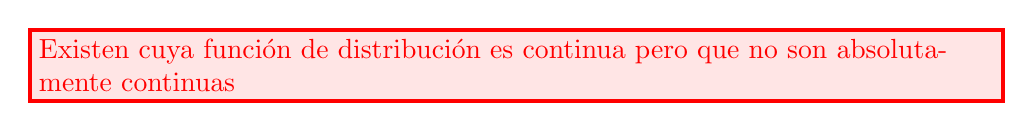
\begin{tikzpicture}
	\node[red, draw=red, fill=red!10, line width=1.5, text width=\textwidth] {Existen \vas cuya función de distribución es continua pero que no son absolutamente continuas};
\end{tikzpicture}

\subsection{Vector aleatorio discreto}
Un vector aleatorio $X$ se dice que es \lb{discreto} si existe un conjunto numerable $\mathcal{S}\in\R^k$ tal que $P(X\in\mathcal{S})=1$.

\lb{Función masa de probabilidad} de una vector aleatorio discreto: \[ P[X=x]=P[X_1=x_1,\dots,X_k=x_k] \]para todo $x=(x_1,\dots,x_k)\in\R^k$, satisfaciendo:
\begin{itemize}[label=$\to$]
\item $P[X=x]\ge0,\;\forall x\in\mathcal{S}$
\item $\sum_{x\in\mathcal{S}}P[X=x]=1$
\end{itemize}
\lb{Función de distribución} de un \vea discreto: \[ F(x)=P[X\le x]= \]

\subsection{Distribuciones marginales}
\subsubsection{Caso continuo}
\begin{itemize}[label=\color{red}\textbullet, leftmargin=*]
	\item \color{lightblue}Distribución marginal de la variable aleatoria $X_i$
\end{itemize}
Sea $X=(X_1,\dots,X_k)$ un \vea continuo con función de densidad $f$ entonces cada componente $X_i$ es de tipo continuo y su función de distribución es; \[ F_{X_i}(x_i)=P[X_i\le x_i]=\int_{-\infty}^{x_i}f_{X_i}(z_i)\mathrm{d}z_i, \]con\[ f_{X_i}=\int_{-\infty}^{+\infty}\cdots\int_{-\infty}^{+\infty}f(z_1,\dots,z_k)\mathrm{d}z_1,\dots, \]

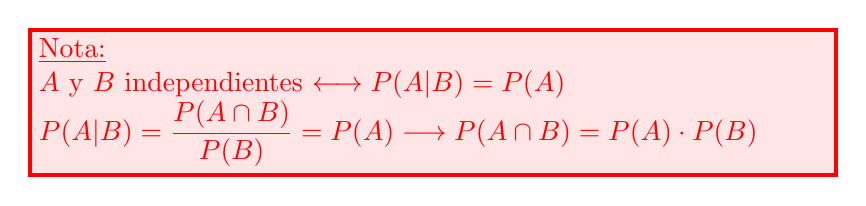
\begin{tikzpicture}
	\node[red, draw=red, fill=red!10, line width=1.5, text width=10cm] {\underline{Nota:}\\
	$A$ y $B$ independientes $\longleftrightarrow P(A|B)=P(A)$\\
	$P(A|B)=\dfrac{P(A\cap B)}{P(B)}=P(A)\longrightarrow P(A\cap B)=P(A)\cdot P(B)$
	};
\end{tikzpicture}

\begin{itemize}[label=\color{red}\textbullet, leftmargin=*]
	\item \color{lightblue}Distribución condicionada al valor de una variable
\end{itemize}

Sea $X=(X_1,\dots,X_k)$

\begin{itemize}[label=\color{red}\textbullet, leftmargin=*]
	\item \color{lightblue}Distribución condicionada a valores de varias variables
\end{itemize}
Sea $X=(X_1,\dots,X_k)$ un vecotr aleatorio continuo

\newpage

\section{Aprendizaje Supervisado}
\subsection{Árboles de Decisión}
\begin{itemize}[label=\color{red}\textbullet, leftmargin=*]
	\item \color{lightblue}Definición
\end{itemize}
Los árboles de decisión son máquinas de aprendizaje supervisado que sirven para clasificar o aproximar.

Supongamos el siguiente problema

\begin{center}
	\begin{tabular}{|c|c|c|c|c|c|}
		\hline
		\rowcolor{lightblue!20}
		\hline
		Paciente & Presión Arterial & Urea en sangre & Gota & Hipotiroidismo & Administrar Tratamiento \\
		\hline
		1 & Alta & Alta & Sí & No & No \\
		\hline
		2 & Alta & Alta & Sí & Sí & No \\
		\hline
		3 & Normal & Alta & Sí & No & Sí \\
		\hline
		4 & Baja & Normal & Sí & No & Sí \\
		\hline
		5 & Baja & Baja & No & No & Sí \\
		\hline
		6 & Baja & Baja & No & Sí & No \\
		\hline
		7 & Normal & Baja & No & Sí & Sí \\
		\hline
		8 & Alta & Normal & Sí & No & No \\
		\hline
		9 & Alta & Baja & No & No & Sí \\
		\hline
		10 & Baja & Normal & No & No & Sí \\
		\hline
		11 & Alta & Normal & No & Sí & Sí \\
		\hline
		12 & Normal & Normal & Sí & Sí & Sí \\
		\hline
		13 & Normal & Alta & No & No & Sí \\
		\hline
		14 & Baja & Normal & Si & Sí & No \\
		\hline
	\end{tabular}
\end{center}
\begin{itemize}
	\item Planteamiento del problema: ¿Cuál es la \textbf{mejor secuencia de preguntas} para saber la clase a la que pertenece un objeto descrito por sus atributos?
	\item Evidentemente, la "mejor respuesta" es aquella que con el \textbf{menor número de preguntas}, devuelve una respuesta suficientemente buena.
	\item ¿Qué es mejor preguntar primero si tiene gota o cómo tiene la presión arterial?
\end{itemize}
\subsubsubsection{Arquitectura}
Un árbol de decisión es una estructura jerárquica que consta de un nodo raíz, ramas, nodos internos y nodos hoja.
\begin{itemize}
	\item Comienzo con un \textbf{nodo raíz} sin ramas entrantes. Las ramas salientes del nodo raíz alimentan los nodos internos.
	\item Los \textbf{nodos internos} evalúan características disponibles para formar subconjuntos homogéneos, indicados por nodos hoja o nodos terminales.
	\item Los \textbf{nodos hoja} representan todos los resultados posibles dentro del conjunto de datos.
\end{itemize}
\begin{center}
	\includegraphics{"Temas/Tema 1/Screenshot002"}
\end{center}
\subsubsubsection{Ventajas y desventajas}
\begin{itemize}[label=\color{lightblue}\textbullet]
	\item Pros
	\begin{itemize}
		\item Fáciles de entender e interpretar.
		\item Sirven también para establecer reglas
		\item No lineales
		\item Menos pre-procesado de los datos: son robustos ante presencia de datos erróneos (outlier), valores faltantes o tipo de datos.
		\item Es un método no paramétrico (por ejemplo, no hay suposición acerca del espacio de distribución y la estructura del clasificador).
	\end{itemize}
	\item Contras
	\begin{itemize}
		\item \textbf{Sobreajuste:} Los árboles más pequeños son más fáciles de interpretar, pero los más grandes pueden resultar en sobreajuste.
		\item Perdida de información al categorizar variables continuas.
		\item \textbf{Precisión:} Otros métodos (por ejemplo, SVM) a menudo tienen tasas de error 30\% más bajas que los árboles básico (ID.3 y CART).
		\item \textbf{Inestabilidad:} un pequeño cambio en los datos puede modificar ampliamente la estructura del árbol (distintos conjuntos, distintos árboles). Varianza elevada.
	\end{itemize}
\end{itemize}
\begin{itemize}[label=\color{red}\textbullet, leftmargin=*]
	\item \color{lightblue}Definición alternativa: \textbf{recursividad}
\end{itemize}
Un árbol de decisión es una estructura recursiva formada por nodos, en el que existe:
\begin{itemize}
	\item Un nodo raíz
	\item El nodo raíz tiene uno o más subnodos.
	\item Cada uno de los subnodos puede ser, a su vez, raíz de un árbol
\end{itemize}
Esta característica recursiva hace que muchos de los algoritmos para crearlos se comporten también de manera recursiva.
\begin{center}
	\includegraphics{"Temas/Tema 1/Screenshot003"}
\end{center}
\subsubsubsection{Clasificación vs Regresión}
\begin{itemize}[label=\color{lightblue}\textbullet]
	\item Clasificación
	\begin{itemize}
		\item La variable dependiente es categórica.
		\item Los valores de los nodos hoja son la \textbf{moda} de las observaciones de la región
	\end{itemize}
	\begin{center}
		\includegraphics{"Temas/Tema 1/Screenshot004"}
	\end{center}
	\item Regresión
	\begin{itemize}
		\item La variable dependiente es continua.
		\item Los valores de los nodos hoja son la \textbf{media} de las observaciones de la región.
	\end{itemize}
	\begin{center}
		\includegraphics{"Temas/Tema 1/Screenshot005"}
	\end{center}
	
\end{itemize}
\subsubsection{Construcción de árboles de decisión}
\subsubsubsection{Particiones}
Cada nodo define una \textbf{partición} del conjunto de entrenamiento en función de los datos que representa.\\
Las particiones producen subconjuntos que son \textbf{exhaustivos} y \textbf{excluyentes}.\\
Cuestiones clave:
\begin{itemize}
	\item \textbf{Tipos de particiones:} cuantos más, más posibilidad de encontrar patrones y, por tanto, los árboles más precisos y expresivos.
	\item \textbf{Número de particiones:} A más particiones mayor complejidad. Equilibrio entre complejidad y precisión.
	\item Selección del \textbf{mejor atributo} en cada paso.
	\item Selección del \textbf{mejor valor} de umbral de los valores.
\end{itemize}
\subsubsubsection{Particiones posibles}
Los algoritmos más populares sólo proponen un tipo de partición para valores nominales y otro para valores numéricos:
\begin{itemize}
	\item \textbf{Particiones nominales:} En el caso que tengamos un atributo $x_i$ que tenga como posibles valores $\{v_1,v_2,\dots,v_n\}$ sólo es posible la partición \[ (x_1=v_1,x_2=v_2,\cdots,x_n=v_n) \]que da lugar a árboles con nodos con más de dos nodos hijos.
	\begin{center}
		\includegraphics{"Temas/Tema 1/Screenshot006"}
	\end{center}
	En el caso de árboles binarios se tienen que evaluar $n$ particiones (una por cada posible valor), definidas por $(x_i=v_i,x_i\neq v_i)$.
	\item \textbf{Particiones numéricas:} Si el atributo $x_i$ es numérico y continuo, se intenta definir particiones que separe las instancias en intervalos de la forma \begin{center}
		$(x_i\le a,x_i>a)$\qquad\begin{minipage}{0.3\textwidth}
			\includegraphics{"Temas/Tema 1/Screenshot007"}
		\end{minipage}
	\end{center}
	eligiendo diferentes valores de $a$ tenemos diferentes particiones. La expresividad resultante se conoce como \textit{expresividad cuadrangular} y que no relacionan atributos (sólo un atributo cada vez).
	\begin{center}
		\includegraphics{"Temas/Tema 1/Screenshot008"}
	\end{center}
	
\end{itemize}
\subsubsection{ID3: Algoritmo básico de aprendizaje}

\begin{quote}
	El algoritmo básico de aprendizaje es el \textbf{ID3 (Iterative Dichotomiser 3)}, J. Ross Quinlan, investigador australiano que propuso el método en 1983
\end{quote}
El método ID3 trata de encontrar una partición que asegure la \textbf{máxima capacidad predictiva y la máxima homogeneidad} de las clases\\
Medida de homogeneidad: la \textbf{entropía}\\
Repetición de \textbf{"cortes en dos"} hasta que se cumpla una determinada condición
\subsubsubsection{Entropía}
Para determinar el mejor atributo, el ID3 utiliza la \textbf{entropía}.

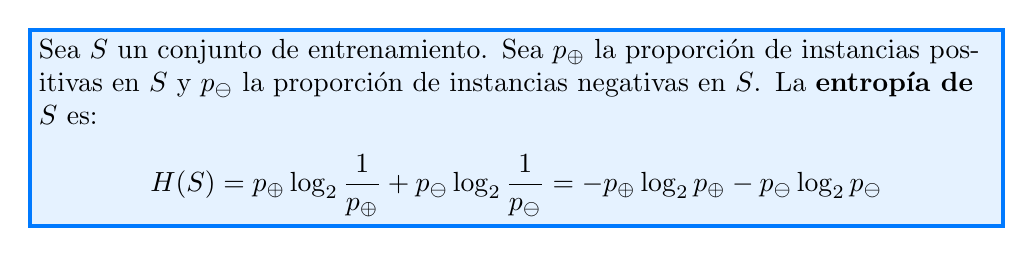
\begin{tikzpicture}
	\node[draw=lightblue, fill=lightblue!10, line width=1.5, text width=\linewidth] {Sea $S$ un conjunto de entrenamiento. Sea $p_\oplus$ la proporción de instancias positivas en $S$ y $p_\ominus$ la proporción de instancias negativas en $S$. La \textbf{entropía de $S$} es: \[ H(S)=p_\oplus\log_2\dfrac{1}{p_\oplus}+p_\ominus\log_2\dfrac{1}{p_\ominus}=-p_\oplus\log_2p_\oplus-p_\ominus\log_2p_\ominus \]};
\end{tikzpicture}

(Relación de la entropía con los conceptos de desorden, equiprobabilidad y homogeneidad).

La entropía nos mide la homogeneidad de los datos (relación inversa).
\begin{center}
	\includegraphics{"Temas/Tema 2/screenshot001"}
\end{center}
\begin{minipage}{0.45\textwidth}
	Para el caso binario:
	\begin{itemize}
		\item Entropía igual a 1 $\to$ mínima homogeneidad (equiprobabilidad: $p_\ominus=p_\oplus$).
		\item Entropía igual a 0 $\to$ máxima homogeneidad (todas las instancias de una clase)
	\end{itemize}
\end{minipage}\qquad\begin{minipage}{0.45\textwidth}
\begin{center}
	\includegraphics{"Temas/Tema 2/screenshot002"}
\end{center}
\end{minipage}
A la hora de construir un árbol es preferible crear nodos con nodos hoja homogéneos, es decir, de \textbf{baja entropía}.
\subsubsubsection{Ganancia de Información}
Sea un conjunto de datos $\mathcal{X}$ con entropía $H(\mathcal{X})$.

Si elegimos un atributo $A$ para crear un nodo del árbol, la entropía esperada es: \[ H(\mathcal{X},A)=\sum_{v\in\mathrm{valores}(A)}\dfrac{|\mathcal{X}_v|}{\mathcal{X}}H(\mathcal{X}_v) \]siendo $\mathcal{X}_v$ el subconjunto de $\mathcal{X}$ con todas las instancias con $A=v$.

Por lo tanto, la reducción esperada de la entropía, o lo que es lo mismo la \textbf{Ganancia de Información}, al elegir el atributo $A$ como nodo de decisión del árbol es \[ \bboxed{\mathrm{Ganacia}(\mathcal{X},A))H(\mathcal{X})-H(\mathcal{X},A)} \]
Por tanto, se elige el atributo que produzca hojas homogéneas, es decir, la \textbf{máxima} ganancia de información.

\Ej

Atributos nominales (no numéricos)

\begin{center}
	\begin{tabular}{|cccccc|}
		\hline
		\rowcolor[HTML]{A5FFC4} 
		\hline
		Día & Cielo & Temperatura & Humedad & Viento & \cellcolor[HTML]{FF8787}Jugar \\ \hline
		\rowcolor[HTML]{34CDF9} 
		\hline
		{\color[HTML]{333333} D1} & {\color[HTML]{333333} Soleado} & {\color[HTML]{333333} Calor} & {\color[HTML]{333333} Alta} & {\color[HTML]{333333} Flojo} & \cellcolor[HTML]{FF8787}No \\
		\rowcolor[HTML]{007AFF} 
		D2 & Soleado & Calor & Alta & Fuerte & \cellcolor[HTML]{FC5D5D}No \\
		\rowcolor[HTML]{34CDF9} 
		D3 & Nublado & Calor & Alta & Flojo & \cellcolor[HTML]{FF8787}Si \\
		\rowcolor[HTML]{007AFF} 
		D4 & Lluvia & Templado & Alta & Flojo & \cellcolor[HTML]{FC5D5D}Si \\
		\rowcolor[HTML]{34CDF9} 
		D5 & Lluvia & Frío & Normal & Flojo & \cellcolor[HTML]{FF8787}Si \\
		\rowcolor[HTML]{007AFF} 
		D6 & Lluvia & Ario & Normal & Fuerte & \cellcolor[HTML]{FC5D5D}No \\
		\rowcolor[HTML]{34CDF9} 
		D7 & Nublado & Ario & Normal & Fuerte & \cellcolor[HTML]{FF8787}Si \\
		\rowcolor[HTML]{007AFF} 
		D8 & Soleado & Templado & Alta & Flojo & \cellcolor[HTML]{FC5D5D}No \\
		\rowcolor[HTML]{34CDF9} 
		D9 & Soleado & Ario & Normal & Flojo & \cellcolor[HTML]{FF8787}Si \\
		\rowcolor[HTML]{007AFF} 
		D10 & Lluvia & Templado & Normal & Flojo & \cellcolor[HTML]{FC5D5D}Si \\
		\rowcolor[HTML]{34CDF9} 
		D11 & Soleado & Templado & Normal & Fuerte & \cellcolor[HTML]{FF8787}Si \\
		\rowcolor[HTML]{007AFF} 
		D12 & Nublado & Templado & Alta & Fuerte & \cellcolor[HTML]{FC5D5D}Si \\
		\rowcolor[HTML]{34CDF9} 
		D13 & Nublado & Calor & Normal & Flojo & \cellcolor[HTML]{FF8787}Si \\
		\rowcolor[HTML]{007AFF} 
		D14 & Lluvia & Templado & Alta & Fuerte & \cellcolor[HTML]{FC5D5D}No \\ \hline
	\end{tabular}
\end{center}
En el ejemplo del tenis tenemos 9 objetos clasificados como $\oplus$ y 5 como $\ominus$, con lo que \[ H([9\oplus,5\ominus])=-0.642\cdot\log_20.642-0.58\cdot\log_20.358=0.94 \]
\begin{center}
	\includegraphics{"Temas/Tema 2/screenshot003"}
\end{center}
Por lo tanto, el atributo que ofrece una mayor ganancia de información es el atributo \textbf{Cielo}.

Utilizando \textbf{Cielo} como nodo raíz el árbol inicial quedaría:
\begin{center}
	\includegraphics{"Temas/Tema 2/screenshot004"}
\end{center}
\begin{minipage}{0.45 \textwidth}
	Ahora habría que repetir el proceso con los nodos correspondientes a los valores \textbf{soleado} y \textbf{lluvia} (el nodo \textbf{nublado} sólo contiene una clase).
\end{minipage}\qquad\begin{minipage}{0.45\textwidth}
\begin{center}
	\includegraphics{"Temas/Tema 2/screenshot005"}
\end{center}
\end{minipage}

\begin{itemize}
	\item Para el nodo Cielo = Soleado:
	\begin{itemize}
		\item $\mathcal{X}_{\mathrm{soleado}}=\{D_1,D_2,D_8,D_9,D_11\}$ con $H(\mathcal{X}_{\mathrm{soelado}})=0.971$
		\item $\mathrm{Ganancia}(\mathcal{X}_{\mathrm{soleado}},\mathrm{Temperatura})=0.971-\dfrac{2}{5}\cdot0-\dfrac{2}{5}\cdot1-\dfrac{1}{5}\cdot0=0.570$
		\item $\mathrm{Ganancia}(\mathcal{X}_{\mathrm{soelado}},\mathrm{Humedad})=0.971-\dfrac{3}{5}\cdot0-\dfrac{2}{5}\cdot0=0.971$
		\item $\mathrm{Ganancia}(\mathcal{X}_{\mathrm{soleado}},\mathrm{Viento})=0.971-\dfrac{2}{5}\cdot1-\dfrac{3}{5}\cdot0.918=0.019$
	\end{itemize}
	\item Para el nodo Cielo = Lluvia:
	\begin{itemize}
		\item $\mathcal{X}_{\mathrm{lluvia}}=\{D_4,D_5,D_6,D_{10},D_{14}\}$ con $H(\mathcal{X}_{\mathrm{lluvia}})=0.971$
		\item $\mathrm{Ganancia}(\mathcal{X}_{\mathrm{lluvia}},\mathrm{Temperatura})=0.971-\dfrac{3}{5}\cdot0.918-\dfrac{2}{5}\cdot1-\dfrac{1}{5}\cdot0=0.820$
		\item $\mathrm{Ganancia}(\mathcal{X}_{\mathrm{lluvia}},\mathrm{Humedad})=0.971-\dfrac{2}{5}\cdot1-\dfrac{3}{5}\cdot0.918=0.820$
		\item $\mathrm{Ganancia}(\mathcal{X}_{\mathrm{lluvia}},\mathrm{Viento})=0.971-\dfrac{3}{5}\cdot0-\dfrac{2}{5}\cdot0=0.971$
	\end{itemize}
\end{itemize}

Por lo tanto, el árbol resultante sería
\begin{center}
	\includegraphics{"Temas/Tema 2/screenshot006"}
\end{center}
Todos los nodos hoja tienen una entropía nula (solo instancias de una clase).
\subsubsubsection{Error global}
Es la probabilidad de error, es decir, suma ponderada de los errores de todas las hojas del árbol. \[ E=\sum_{i=1}^{n_h}w_ie_i \]donde
\begin{itemize}
	\item $n_h$ es el numero de hojas del árbol.
	\item $w_i$ es el peso o probabilidad de la hoja $i$, es decir, la probabilidad de que una instancia sea clasificada por la partición representada por la rama que acaba en la hoja $i$.
	\item $e_i$ es el error correspondiente a la rama que acaba en la hoja $i$ (número de instancia erróneas que caen en la hoja $i$ entre el número de instancias que caen en la hoja $i$).
\end{itemize}
\subsubsubsection{Algoritmo}
El algoritmo básico de aprendizaje es el ID3 (Iterative Dichotomiser 3).

\begin{algorithm}
	\caption{árbol $\gets$ aprenderArbol(\textit{datos})}
	\begin{algorithmic}[1]
		\IF{todos los ejemplos en datos tienen la misma etiqueta}
		\RETURN un nodo hoja con dicha etiqueta
		\ELSE
		\STATE Sea $A$ el atributo que clasifica mejor a los objetos en datos
		\FORALL{posible valor $v$ de $A$}
		\STATE $data(v) \leftarrow$ todos los objetos con $A = v$
		\STATE Añadir nueva rama $\leftarrow$ aprenderArbol($data(v)$)
		\ENDFOR
		\RETURN árbol
		\ENDIF
	\end{algorithmic}
\end{algorithm}

\pagebreak

\textbf{ID3(Instancias, Etiquetas, Atributos)}

\begin{algorithmic}
	\REQUIRE \texttt{Instancias:} el conjunto de datos
	\REQUIRE \texttt{Etiquetas:} el conjunto de posibles clases.
	\REQUIRE \texttt{Atributos:} el conjunto de atributos en el conjunto \texttt{Instancias}.
	\IF{todas las instancias son positivas}
	\RETURN el nodo raíz con etiqueta $+$.
	\ELSIF{todas las instncias son negativas}
	\RETURN el nodo raíz con la etiqueta $-$.
	\ELSIF{\texttt{Atributos}=$\varnothing$}
	\RETURN el nodo raíz con el valor de \texttt{Etiquetas} más probable en \texttt{Instancias}.
	\ENDIF
	\STATE Sea $A$ el atributo que clasifica mejor las instancias en \textit{datos}.
	\STATE Crear un árbol con un nodo etiquetado con $A$
	\FORALL{posible valor $v_i$ del atributo $A$}
	\STATE añadir un arco bajo la raíz con la comprobación $A=v_i$.
	\STATE sea \texttt{Instancias} $v_i$ el subconjunto de \texttt{Instancias} con $A=v_i$.
	\IF{\texttt{Instancias}$_{v_i}=\varnothing$}
	\STATE añadir un nodo hoja al arco añadido con el valor de \texttt{Etiquetas} más probable en \texttt{Ejemplos}.
	\ELSE 
	\STATE añadir al nuevo árbol el subárbol generado por \textbf{ID3} (\texttt{Instancias}$_{v_i}$,\texttt{Etiquetas}, \texttt{Atributos}$-\{A\}$).
	\ENDIF
	\ENDFOR
	\RETURN nodo raíz
\end{algorithmic}
\subsubsection{Sobre-ajuste}
\subsubsubsection{Espacio de hipótesis y sobre-ajuste}
El \textbf{espacio de hipótesis} $H$ (no confundir con la entropía) en árboles de decisión
abarca todas las posibles combinaciones de atributos y valores que pueden formar
árboles de decisión, y nuestra tarea es encontrar la hipótesis más adecuada para
clasificar correctamente las instancias de entrada.

En general, se prefieren hipótesis cortas para evitar el sobre-ajuste (\textbf{overfitting}).

\begin{itemize}[label=\color{red}\textbullet, leftmargin=*]
	\item \color{lightblue}Sobre-ajuste
\end{itemize}
Dado un espacio de hipótesis $H$, se dice que una hipótesis particular $h\in H$ sobreajusta los datos de entrenamiento si existe un hipótesis alternativa $h'\in H$, tal que $h$ presenta un error menor que $h'$ sobre los ejemplos de entrenamiento, pero $h'$ presenta un error menor que $h$ sobre el conjunto total de observaciones.
\subsubsubsection{Proceso de poda}
\begin{itemize}[label=\color{red}\textbullet, leftmargin=*]
	\item \color{lightblue}¿Cómo podemos evitar el sobre-aprendizaje o sobre-ajuste?
\end{itemize}
\textbf{Poda:} Eliminar condiciones de las ramas del árbol encontrar más pequeños. Existe dos tipos de poda:\begin{itemize}
	\item \textbf{Prepoda:} El proceso se realiza durante la construcción del árbol, estableciendo un criterio de parada.
	\begin{itemize}
		\item El número de instancias por nodo.
		\item El error esperado.
		\item MDL (Minimun Description Lenght).
	\end{itemize}
	\item \textbf{Postpoda:} El proceso se realiza después de la construcción del árbol
	\begin{itemize}
		\item Consiste en ir eliminando nodos de abajo a arriba mientras se vaya cumpliendo un criterio determinado.
	\end{itemize}
\end{itemize}
Se pueden combinar ambas aproximaciones.
\subsubsubsection{Otras medidas}
\textbf{Medidas alternativas:} En algunos casos se suele utilizar otras medidas como:
\begin{itemize}
	\item El \textit{Ratio} de la ganancia de información, para evitar el hecho de que se favorece la selección de los atributos con más valores.
	\item MSE para regresión
	\item Índice Gini empleado por el algoritmo CART
	\item DKM, basados en AUC, MDL
\end{itemize}
\subsubsection{Algoritmo CART y Otros}
\subsubsubsection{CART}
\textbf{Cart} (\textbf{C}lasificación \textbf{A}nd \textbf{R}egression \textbf{T}rees). Similar al ID3 pero:
\begin{itemize}
	\item Permite que la variable que define la clase sea continua y no construye un conjunto de reglas.
	\item Utiliza el índice de Gini en vez de la ganancia de información para seleccionar el mejor atributo (la mejor partición).
	\item Utiliza también el esquema de partición recursiva utilizando una estrategia voraz.
	\item También permite resolver problemas de regresión.
\end{itemize}
Se elige la partición que produce el menor valor de la función de coste.
\begin{itemize}
	\item Para regresión: RSME.
	\item Para clasificación: GINI \[ \mathrm{Gini}(p)=\sum_{i=1}^{n}p_i(1-p_i) \] con $p_i$ las proposiciones de instancias de la clase $i$ en la partición.
\end{itemize}
Prepoda: Utiliza como criterio de parada el número mínimo de instancias asignadas al nodo.

Postpoda: Utiliza un criterio que controla la importancia relativa del error frente la complejidad (tamaño del árbol).
\subsubsubsection{C4.5, C5.0}
\textbf{C4.5:} Permite, a diferencia que ID3, que las características puedan ser continuas, definiendo de forma dinámica un atributo discreto particionando los atributos continuos en un conjunto discreto de intervalos.
\begin{itemize}
	\item C4.5 transforma los árboles obtenidos en un conjunto de reglas del tipo \textit{if-then}. La precisión de cada regla es evaluada de forma independiente para determinar el orden en el que deben ser aplicadas.
	\item Un proceso de poda elimina antecedentes de las reglas si con esto se mejora la precisión de la misma.
	\item C5.0, utiliza menos memoria y obtiene un conjunto de reglas menor y más preciso.
	\item J48 es la implementación en código abierto de C4.5
\end{itemize}
\subsubsection{Random Forests}
Random Forest es una técnica que construye un gran número de árboles de decisión no correlacionados.

Se basa en la técnica de Agregación de Bootstrap (Bagging), técnica de agregación de clasificadores o regresores que:
\begin{itemize}
	\item Aumenta la precisión y estabilidad reduciendo los efectos del ruido.
	\item Reduce la varianza en las predicciones.
	\item Ayuda a evitar el sobre ajuste.
\end{itemize}
La predicción del modelo se elige analizando las predicciones de cada uno de los árboles considerados en el modelo.
\subsubsubsection{Algoritmo}
\begin{algorithm}
	\caption{RF $\gets$ RandomForest(\textit{datos})}
	\begin{algorithmic}[1]
		\FOR{$i\gets1\to$ \textit{n_arboles}}
		\STATE Extraer una muestra de tamaño \textit{size(data)} de \textit{datos} por bootstrapping
		\STATE Construir un árbol $T_i$ repitiendo recursivamente para cada nodo hoja
		\STATE \begin{enumerate}[leftmargin=1.5cm]
			\item Seleccionar aleatoriamente $m$ atributos.
			\item Seleccionar la mejor partición de las inducidas por los $m$ atributos.
			\item Dividir el nodo en dos nodos hijos.
			\item Si el tamaño de nodo alcanza $n_{\min}$ no continuar dividiendo.
		\end{enumerate}
		\ENDFOR
		\RETURN El conjunto de árboles $\{T_i\}_1^{\text{\textit{n_arboles}}}$.
	\end{algorithmic}
\end{algorithm}

Si tenemos $p$ atributos las recomendaciones para el valor de $m$ son:
\begin{itemize}
\item Clasificación: $\lfloor\sqrt{m}\rfloor$

\item Regresión: $\lfloor p/3\rfloor$
\item Siendo el valor mínimo 1.
\end{itemize}
Una vez se han construido los árboles para hacer predicciones:
\begin{itemize}
	\item Clasificación: La clase más votada por los árboles.
	\item Regresión: La media de todas las predicciones
\end{itemize}
\subsubsubsection{OBB e importancia de las variables}
\textbf{OBB (out of the bag) error estime:} Para cada muestra se predice el error utilizando sólo los árboles en los que no ha sido utilizada (no ha sido elegida en bootstrapping)
\begin{itemize}
	\item Los valores son parecidos a los que se obtienen mediante una validación cruzada de $N$-pliegues.
\end{itemize}
\textbf{Importancia de los atributos:}
\begin{itemize}
	\item En cada partición del árbol se registra la mejora del criterio de división.
	\item Este valor se considera la importancia del atributo.
	\item Para cada variable se agregan los valores generados en cada árbol.
\end{itemize}
\subsubsection{Conclusiones}
La utilización de árboles de decisión es muy popular en muchas disciplinas.

Experimentalmente han demostrado una buena capacidad de clasificación.

La clave reside en la función a optimizar a la hora de elegir el atributo para disgregar el árbol.

Los ensambles nos permiten mejorar los resultados combinando información.
\subsubsection{Bosques Aleatorios (\textit{"Random Forest"})}
\subsubsubsection{Motivación}
Surgen para resolver el \textbf{"overfitting"} producido por los árboles de decisión.

El gran problema de los árboles de decisión: sesgo bajo y varianza alta.

Cambios imperceptibles en la distribución de los datos modifican totalmente la partición generada por un Árbol de Decisión (varianza alta).

\begin{center}
	\includegraphics{"Temas/Tema 2/screenshot007"}
	
	¿Cómo reducir la varianza?
\end{center}
\subsubsubsection{Solución}

\textbf{Muchos árboles} de decisión

\textbf{Aleatoriedad doble}
\begin{itemize}
	\item Conjuntos de entrenamiento 
\item Características 
\end{itemize}
\textbf{Agregación} de resultados 
\begin{itemize}
	\item Árboles malos, poco impacto en la predicción
\end{itemize}
\begin{center}
	\includegraphics{"Temas/Tema 2/screenshot008"}
	
	\includegraphics{"Temas/Tema 2/screenshot009"}
\end{center}
\subsubsubsection{Número de árboles}

\begin{minipage}{0.5\textwidth}
	Lo primero es fijar el \textbf{número de árboles}
	\begin{itemize}
		\item Normalmente es elevado, cientos.
	\item En este ejemplo, \textbf{5}
	\end{itemize}
	
	\hspace{2cm}
	
	Ruido en los datos afectará a algunos árboles
\end{minipage}\quad\begin{minipage}{0.5\textwidth}
\begin{center}
	\includegraphics[width=\linewidth]{"Temas/Tema 2/screenshot010"}
\end{center}
\end{minipage}
\subsubsubsection{Generación conjuntos de entrenamiento}
\begin{minipage}{0.5\textwidth}
\begin{center}
Una vez fijado el \textbf{número de árboles}, se construyen los conjuntos de entrenamiento.
	
	\begin{tikzpicture}
		\draw[double -latex=4pt colored by lightblue and lightblue] (0,0) -- (0,-1);
	\end{tikzpicture}
	
	{\Large \lb{\textbf{BOOSTRAPPING}}}
	
	Muestreo con reemplazo
\end{center}
\begin{itemize}[label=\color{red}\textbullet, leftmargin=*]
	\item \color{lightblue}Obtención de muestras \textbf{“Bootstrap”}
\end{itemize}

Supongamos un conjunto de datos $X$ (población) de tamaño $N$.
Se construyen muestras bootstrap de la población a partir de los datos:
\begin{enumerate}[label=\color{lightblue}\arabic*)]
	\item Elegir el tamaño de la muestra $N'\le N$.
	\item For $i=1:N'$
	\begin{enumerate}[label=\color{lightblue}\arabic*)]
		\item Elegir aleatoriamente una observación de $X$ con \textit{reemplazo}
		\item Añadirlo a la muestra
	\end{enumerate}
\end{enumerate}
En machine learning, $N'=N$.
\end{minipage}\qquad\begin{minipage}{0.45\textwidth}
\begin{center}
	\includegraphics[width=\linewidth]{"Temas/Tema 2/screenshot011"}
\end{center}
\end{minipage}
\begin{center}
	\includegraphics{"Temas/Tema 2/screenshot012"}
\end{center}

\subsubsubsection{Entrenamiento de los árboles}
Se introduce una \lb{segunda aleatoriedad} en la selección de las características que se emplean para realizar las particiones.
\begin{center}
	\includegraphics{"Temas/Tema 2/screenshot013"}
\end{center}

\begin{minipage}{0.5\textwidth}
	De la misma forma, se van entrenando (y construyendo) los demás árboles
\end{minipage}\quad\begin{minipage}{0.5\textwidth}
\begin{center}
	\includegraphics[width=\linewidth]{"Temas/Tema 2/screenshot014"}
\end{center}

\end{minipage}
\subsubsubsection{Modo operación}
\begin{center}
	\includegraphics{"Temas/Tema 2/screenshot015"}
\end{center}
\subsubsubsection{Bagging y Conjunto de Validación}

\textbf{Bagging:} es la la combinación del bootstrapping y la agregación, que es precisamente el nombre genérico con que se conoce a los algoritmos como los Bosques Aleatorios y otros similares.

\lb{\textbf{Conjunto de validación o "out-of-bag":}} se emplea para selección de hiperparámetros
\begin{center}
	\begin{tabular}{rl}
		$\dfrac{1}{N}$ & $\to$ probabilidad de seleccionar una instancia\\
		$1-\dfrac{1}{N}$ & $\to$ probabilidad de que no se seleccione una instancia\\
		$\left(1-\dfrac{1}{N}\right)^N\approx e^{-1}=0.368$ & $\to$ probabilidad que una instancia no se seleccione tras $N$ veces
	\end{tabular}
	
	\begin{tabular}{ll}
		Por tanto, aproximadamente: & conjunto de \textbf{validación} ("out-of-bag") $\to 36.8\%$\\
		&conjunto de \textbf{entrenamiento} $\to63.2\%$
	\end{tabular}
\end{center}
\subsubsubsection{Selección del número de árboles}
\begin{minipage}{0.4\textwidth}
Se fija el número de características y el criterio de parada, y se entrenan múltiples bosques cambiando progresivamente el número de árboles que lo conforman.

Se selecciona el que menor error de validación proporciona.

Usualmente, en aplicaciones prácticas, se usan entre 100 y 200 árboles
\end{minipage}\qquad\begin{minipage}{0.55\textwidth}
\begin{center}
	\includegraphics[width=\linewidth]{"Temas/Tema 2/screenshot016"}
\end{center}

\end{minipage}
\subsubsubsection{Seleccionar del número de características}
\begin{minipage}{0.4\textwidth}
	Con el número de árboles ya
	determinado, fijamos el
	criterio de parada y repetimos
	el procedimiento cambiando
	el número de características, y
	escogemos aquel que genere
	el menor error.
\end{minipage}\qquad\begin{minipage}{0.55\textwidth}
\begin{center}
	\includegraphics[width=\linewidth]{"Temas/Tema 2/screenshot017"}
\end{center}

\end{minipage}
\subsubsubsection{Selección del criterio de parada}
\begin{minipage}{0.4\textwidth}
Finalmente, con el número de árboles
y de características fijo, variamos el
criterio de parada y escogemos el que
arroje el menor error. El criterio de
parada puede ser, por ejemplo, el
mínimo número de datos de una hoja
(algún método de prepoda).
\end{minipage}\qquad\begin{minipage}{0.55\textwidth}
\begin{center}
	\includegraphics[width=\linewidth]{"Temas/Tema 2/screenshot018"}
\end{center}

\end{minipage}
\subsubsubsection{Relevancia de las características}
\begin{minipage}{0.5\textwidth}
	Los valores de los índice Gini (para el caso de la clasificación)
o el error cuadrático medio (para el caso de la regresión)
aportan una medida de la bondad de la partición hecha en
cada nodo. Con estos valores, se puede establecer un \textbf{orden de importancia} de las características. 
\end{minipage}\qquad\begin{minipage}{0.5\textwidth}
\begin{center}
	\includegraphics[width=\linewidth]{"Temas/Tema 2/screenshot019"}
\end{center}
\end{minipage}
\begin{center}
	\includegraphics{"Temas/Tema 2/screenshot020"}
\end{center}
\subsection{Perceptrón monocapa y multicapa (MLP)}
\subsubsection{Teoría de la decisión}
Tres escenarios para resolver un problema de decisión
\begin{itemize}
	\item \textbf{Decisión analítica.} Se fundamentan en la teoría bayesiana para inferir las probabilidades a posteriori de las las clases
	\item \textbf{Modelos discriminatorios.} Infieren directamente las probabilidades a posteriori.
	\item \textbf{Funciones discriminantes.} Encuentran una función $f(x)$ que mapea directamente una entrada $x$ a una determinada clase.
\end{itemize}
\subsubsubsection{Decisión analítica}
Se fundamentan en la inferencia de $p(\mathrm{x}|C_k)$ y $p(C_k)$ (o, equivalente $p(\mathbf{x},C_k)$).

\begin{minipage}{0.5\textwidth}
	Procedimiento:
	\begin{enumerate}[label=\color{lightblue}\arabic*)]
		\item A partir de los datos, se infieren verosimilitudes y probabilidades a priori: $p(\mathbf{x}|C_k)$ y $p(C_k)$.
		\item Se aplica el Teorema de Bayes para calcular las probabilidades a posteriori \[ p(C_k|\mathrm{x})=\dfrac{p(\mathrm{x}|C_k)p(C_k)}{p(\mathrm{x})}=\dfrac{p(\mathrm{x}|C_k)p(C_k)}{\displaystyle\sum_kp(\mathrm{x}|C_k)p(C_k)} \]
		\item Se emplea la teoría de la decisión para determinar la clase de una entrada $x$
	\end{enumerate}
	Los métodos que explícita o implícitamente modelan las distribuciones de las entradas así como las salidas, $p(\mathrm{x},C_k)$, se llaman \textbf{modelos generativos} pues mediante \textit{muestreo} se pueden generar datos sintéticos.
\end{minipage}\qquad\begin{minipage}{0.5\textwidth}
\begin{center}
	\includegraphics{"Temas/Tema 2/screenshot021"}
\end{center}
\end{minipage}
\subsubsubsection{Modelos discriminatorios}
Producen directamente una estima de las probabilidades a posteriori de las clases para una entrada dada.
\begin{enumerate}[label=\color{lightblue}\arabic*)]
	\item El procedimiento ahora consiste en, con los datos disponibles, diseñar y entrenar un modelo que minimice una determinada función de error entre las entradas y sus salidas deseadas
	\item Las salidas del modelos representan, mediante algún código, las probabilidades a posteriori de las clases para la entrada dada.
	\item El ejemplo más claro de modelos discriminativos son las \textbf{redes neuronales progresivas} como, por ejemplo, los MLPs entrenados para minimizar la entropía cruzada con unidades de salida tipo softmax
\end{enumerate}
\begin{center}
	\includegraphics{"Temas/Tema 2/screenshot022"}
\end{center}
\subsubsubsection{Funciones discriminantes}
Encuentran una función $f(x)$, llamada \textit{función discriminante}, que directamente mapea cada entrada $x$ a la etiqueta de una clase.

\begin{minipage}{0.5\textwidth}
	\begin{itemize}[label=\color{red}\textbullet, leftmargin=*]
		\item \color{lightblue}Ejemplo: problema de dos clases
	\end{itemize}
	\[ \begin{array}{ll}
		f(x)=1, & \text{si }y(x)=\mathrm{w}^\intercal\mathrm{x}+w_0>0\\
		f(x)=0, & \text{si }y(x)=\mathrm{w}^\intercal\mathrm{x}+w_0<0
	\end{array} \]
\end{minipage}\qquad\begin{minipage}{0.5\textwidth}
\begin{center}
	\includegraphics[width=\linewidth]{"Temas/Tema 2/screenshot023"}
\end{center}

\end{minipage}
\subsubsection{Fundamento biológico}
Membrana permeable para ciertas sustancias iónicas. Se crea una diferencia de potencial.

\begin{center}
	\includegraphics{"Temas/Tema 2/screenshot024"}
\end{center}
Tras la activación sináptica, se propagan diferencias de potencial.entre el soma y el entorno.
\begin{center}
	\includegraphics{"Temas/Tema 2/screenshot025"}
\end{center}
\subsubsection{Perceptrón monocapa}
\subsubsubsection{(Widrow): filtro transversal (adaptativo) + umbral duro}
\begin{center}
	\includegraphics{"Temas/Tema 2/screenshot026"}
\end{center}
\begin{minipage}{0.5\textwidth}
	División según hiperplano: \[ z=\mathbf{w^\intercal x}+b=0 \]donde la \lb{Función discriminante} (lineal) es \[ z=\mathbf{w^\intercal x}+b \]
\end{minipage}\qquad\begin{minipage}{0.5\textwidth}
\begin{center}
	\includegraphics{"Temas/Tema 2/screenshot027"}
\end{center}
\end{minipage}
\subsubsubsection{(Rosenblatt): dados $N$ pares entrada-salida: $\{\mathbf{x}_k,\mathbf{d}_k\}_1^N$}
Muestra a muestra: \[ \mathbf{w}(k+1)=\mathrm{w}(k)+\dfrac{\alpha}{2}(d_k-o_k)x_k,\quad(\alpha>0) \]
Bloque: \[ \mathrm{w}(m+1)=\mathrm{w}(m)=\dfrac{\alpha}{2}\sum_{k=1}^{N}(d_k-o_k(m))\mathrm{x}_k,\quad(\alpha>0) \]
Es aprendizaje:
\begin{itemize}
	\item \textbf{Supervisado:} pares de entrenamiento dados.
	\item \textbf{No lineal:} se emplea la salida $(o)$ en el error.
	\item \textbf{Hebbiano:} refuerza las intervenciones correctas ($\pm\alpha\mathrm{x}_k$ en $\mathbf{w}$ según el signo del error).
\end{itemize}
Solo converge si hay separabilidad lineal

Ejemplo gráficos: $D=2,b=0$ y una muestra $\{\mathbf{x}_k,\lbb{d_k=-1}{\text{salida deseada}}\}$
\begin{center}
	\includegraphics[width=\linewidth]{"Temas/Tema 2/screenshot028.drawio"}
\end{center}

Las rectas narajas y amarillan se sacan sumando a $\mathrm{w}(k+1)$ y $\mathrm{w}(\alpha)$ respectivamente el $-\alpha x$.

Es decir, aplicando la fórmula de muestra a muestra.
\subsubsection{Limitaciones del Perceptron Monocapa}
Minskey y Papert: es un "solo" \textbf{discriminante lineal}, capaz de resolver problemas de juguete (por ejemplo OREX).
\begin{center}
	\includegraphics{"Temas/Tema 2/screenshot029"}
\end{center}
Si se dispone en capas: gradiente imposible por el umbral duro.

La ya comentada falta de convergencia.
\subsubsection{El algoritmo LMS}
(Widrow y Hopf): proponen emplear $z$ en el error en lugar de $o$ y minimizar el coste cuadrático (Least Mean Square) por gradiente: \[ \min_{\mathrm{x}}C(\mathrm{w})=\min_{\mathrm{w}}\dfrac{1}{2}\sum_{k=1}^{N}(d_k-z_k)^2 \]
\begin{itemize}
	\item Muestra a muestra: \[ \mathrm{w}(k+1)=\mathrm{w}(k)+\alpha(d_k-z_k)\mathrm{x}_k,\quad(\alpha>0) \] (más rápido, pero más ruidoso).
	\item Bloque: \[ \mathrm{w}(m+1)=\mathrm{w}(m)+\alpha\sum_{k=1}^{N}(d_k-z_k(m))\mathrm{x}_k,\quad(\alpha>0) \]
\end{itemize}

Para entradas independientes de valores independientes de media cero y autocorrelación $R_{\mathrm{xx}}$, converge a la solución MMSE (solución de Wiener-Hopf) \[ \mathrm{x}_{opt}=R_{xx}^{-1}\mathtt{E}\{\dx\}\text{ si }\alpha<\dfrac{2}{\lambda_{\max}} \]
\subsubsection{Características del LMS}
El LMS es muy robusto: converge en muchos casos

Aprendizaje:
\begin{itemize}
	\item \textbf{Supervisado}
	\item \textbf{Lineal:} se emplea la salida $(\mathbf{z})$ en el error
	\item Por prestaciones: según coste cuadrático
\end{itemize}
Produce resultados razonables (los mejores mediante una frontera lineal) aunque el problema no se separable linealmente.

\textbf{NLMS ó Delta-LMS:} $\alpha\longrightarrow\dfrac{\alpha}{\|\mathbf{x}\|^2}$, independiza de la energía de las muestras.
\subsubsection{Error cuadrático (SSE) para clasificación}
\subsubsubsection{Problema con los "OUTLIERS"}
\begin{center}
	\includegraphics{"Temas/Tema 2/screenshot030"}
\end{center}
La figura muestra el resultado obtenido por el LMS (en morado) para dos situaciones distintas.
\subsubsection{Activación blanda}
El \textbf{umbral duro} de Widrow, se cambia por una \textbf{aproximación derivable}

Resulta adecuada la forma sigmoidal o sigmoide:

\begin{minipage}{0.5\textwidth}
	\begin{itemize}
		\item \textbf{Función logística:} \[ o=f(z)=\dfrac{1}{1+e^{-gz}} \]
		\item \textbf{Tangente hiperbólica} ($\tanh$): \[ o=f(z)=\dfrac{1-e^{-gz}}{1+e^{-gz}}=\tanh\left(\dfrac{gz}{2}\right) \]
	\end{itemize}
\end{minipage}\qquad\begin{minipage}{0.5\textwidth}
\begin{center}
	\includegraphics[scale=0.8]{"Temas/Tema 2/screenshot031"}
\end{center}
\end{minipage}

$g$: saturación (determina la pendiente de la sigmoide en $z=0$).

En principio, asumible por los pesos.
\subsubsection{LMS con activación blanda}
Ahora: $z\to o$: \[ \min_{\mathrm{w}}C(\mathrm{w})=\min_{\mathrm{w}}\dfrac{1}{2}\sum_{k=1}^{N}(d_k-o_k)^2 \]
\begin{itemize}
	\item Muestra a muestra: \[ \mathrm{w}(k+1)=\mathrm{w}(k)+\alpha(d_k-o_k)f'(z_k)\mathrm{x}_k,\quad(\alpha>0) \]
	\item Bloque: \[ \mathrm{w}(m+1)=\mathrm{w}(m)+\alpha\sum_{k=1}^{N}(d_k-o_k(m))f'(z_k(m))\mathrm{x}_k,\quad(\alpha>0) \]
\end{itemize}
Aparece un factor $f'(z_k)$ que se puede calcular a partir de la propia salida según:

\begin{minipage}{0.5\textwidth}
	\begin{itemize}
		\item Para función logística: $f'(z)=go(1-o)$
	
	\[ \begin{aligned}
		\text{Demo: }f'(z)&=\dfrac{ge^{-gz}}{(1+e^{-gz})^2}=g\dfrac{1}{(1+e^{-gz})}\dfrac{e^{-gz}}{(1+e^{-gz})}\\
		&=g\dfrac{1}{(1+e^{-gz})}\left(1-\dfrac{1}{(1+e^{-gz})}\right)\\
		&=go(1-o)
	\end{aligned} \]
	\item Para $\tanh:\:f'(z)=\dfrac{1}{2}g(1-o^2)$
	\end{itemize}
\end{minipage}\qquad\begin{minipage}{0.5\textwidth}
\begin{center}
	\includegraphics{"Temas/Tema 2/screenshot031"}
\end{center}
\end{minipage}
\subsubsection{Arquitectura del Perceptron Multicapa (MLP)}
\subsubsubsection{Redes Multicapa}
\begin{center}
	\includegraphics{"Temas/Tema 2/screenshot032"}
\end{center}
\subsubsection{Propiedades de las MLP}
Son:
\begin{itemize}
	\item potentes
	\item versátiles
	\item distribuidas: robustas
	\item paralelas: rápidas (entrenadas)
\end{itemize}
pero:
\begin{itemize}
	\item de entrenamiento difícil y lento
	\item de difícil análisis
\end{itemize}
\subsubsection{Capacidades del MLP}
\begin{center}
	\includegraphics[width=\linewidth]{"Temas/Tema 2/screenshot033"}
\end{center}
Para MLPs con dos capas ($L = 2$), se han probado los siguientes teoremas:

Cybenko: basta con una capa oculta de unidades sigmoidales (en número indefinido) para \begin{center}
	$R^{N_0}\longrightarrow(1,-1)^{N_L}$\quad(Clasificación)
\end{center} donde $N_0$ y $N_L$ son la dimensión de la entrada y la salida, respectivamente.

Kolmogorov (adaptado por Hetch-Nielsen): basta con una capa oculta de $2N_0 + 1$ unidades de activaciones adecuadas para \begin{center}
	$(1,-1)^{N_0}\longrightarrow R^{N_L}\quad$(Regresión)
\end{center}
\subsubsection{Notación utilizada MLP}
\begin{center}
	\includegraphics{"Temas/Tema 2/screenshot034"}
\end{center}
\subsubsection{Algoritmo de retropropagación (BackPropagation (BP))}
Básicamente consiste en dos fases:
\begin{itemize}
	\item \textbf{Hacia adelante:} primero se aplica una instancia a las entradas de la red y su efecto se propaga a través de la misma, capa a capa, hasta la salida.
	\item \textbf{Hacia atrás (BP):} Después, se re-calculan los pesos mediante el gradiente del error. En concreto, se calcula el valor de la función de error, que compara la respuesta actual de la red y la respuesta deseada, y este error se propaga hacia atrás.
\end{itemize}
El objetivo es minimizar \[ \min_{\mathrm{w}}C(\mathrm{w})=\min_{\mathrm{w}}\dfrac{1}{2}\sum_{m=1}^{N}(\mathbf{d}_m-\mathbf{o}_m)^2 \] donde $\mathbf{w}$ representa todos los pesos de la red y $m$ la muestra o instancia.

Algoritmo de gradiente \[ w_{ji}^{(l)}(k+1)=e_{ji}^{(l)}(k)-\eta\dfrac{\partial C}{\partial w_{ji}^{(l)}}(k) \]
Para cada iteración $k$, se tienen las ecuaciones siguientes $\dfrac{\partial C}{\partial w_{ji}^{(l)}}=\dfrac{\partial C}{\partial o_j^{(l)}}\dfrac{\partial o_j^{(l)}}{\partial w_{ji}^{(l)}}=\dfrac{\partial C}{\partial o_j^{(l)}}f_j^{\prime(l)}o_i^{(l-1)}=\Delta_j^{(l)}o_i^{(l-1)}$ ya que \linebreak $o_j^{(l)}=f\left(\sum_{k=1}^{N_{l-1}}e_{jk}^{(l)}o_k^{(l-1)}\right)$
\begin{equation}
	\begin{split}
	\Delta_j^{(l)}&=\left(\sum_{n_{l+1}}^{N_{l+1}}\dfrac{\partial C}{\partial o_{n_{l+1}}^{(l+1)}}\dfrac{o_{n_{l+1}}^{(l+1)}}{\partial o_j^{(l)}}\right)f_j^{\prime(l)}=\left(\sum_{n_{l+1}}^{N_{l+1}}\dfrac{\partial C}{\partial o_{n_{l+1}}^{(l+1)}}f_{n_{l+1}}^{\prime(l+1)}w_{n_{l+1}j}^{(l+1)}\right)f_j^{\prime(l)}\\
	&=\left(\sum_{n_{l+1}}^{N_{l+1}}\Delta_{n_{l+1}}^{(l+1)}w_{n_{l+1}j}^{(l+1)}\right)f_j^{\prime(l)}
\end{split}
\end{equation}
BackPropagation (también Regla Delta Generalizada)) \[ w_{ji}^{(l)}(k+1)=w_{ji}^{(l)}-\eta\Delta_j^{(l)}(k)o_i^{(l-1)}(k) \]
Se procede: \[ l=L\longrightarrow L-1,L-2,\dots,1\quad\text{(¡retroprogramación!)} \] insertando gradiente y considerando que
\begin{itemize}
	\item Para $l=L$ se aplica \[ \Delta_j^L=\dfrac{\partial C}{\partial o_j^{(L)}}f_j^{\prime (L)} \]
	\item Y para $l<L$, se aplica (1)
\end{itemize}
Recuérdese que, para sigmoides, las derivadas dependen solo de los salidas: $f'(z)=go(1-o)$ para función logística y $f'(z)=\dfrac{1}{2}g(1-o^2)$ para $\tanh$.
\subsubsection{Modos de entrenamiento}
\begin{itemize}[label=\color{red}\textbullet, leftmargin=*]
	\item \color{lightblue}¿Cada cuanto se actualizan los pesos?
\end{itemize}
\begin{itemize}
	\item \lb{Batch:} depués de cada época del conjunto de entrenamiento.
	\item \lb{Mini-Batch:} despuñes de una muestra (conjunto de patrones) del conjunto de entrenamiento.
	\item \lb{Online:} depués de cada ejemplo.
\end{itemize}
\begin{center}
	\includegraphics{"Temas/Tema 1/Screenshot030"}
\end{center}
\subsubsection{Sobre las muestras}
Conjunto de muestras de entrenamiento \lb{representativo}

Conviene \lb{preprocesar} las muestras para eliminar información que de seguro se sabe irrelevante

Conviene \lb{normalizar} (características con media nula y varianza unidad)

Pueden ser útiles \lb{códigos sencillos} (en general, las NNs muestran sensibilidad al formato de presentación). Ejemplos: 1:N, termómetro, etc.

Para el mini-batch y online, conviene \lb{Aleatorizar} el orden de presentación de las muestras y \lb{ciclar} las series de entrenamiento.

\newpage

\section{El concepto de integral de Riemann y sus propiedades}
\subsection{Función integrable}
\begin{itemize}[label=\color{red}\textbullet, leftmargin=*]
	\item \color{lightblue}Definición
\end{itemize}
Dado $[a,~b]$ un intervalo de la recta real, se define una partición $\mathcal{P}$ de dicho intervalo como una sucesión finita de números reales de la forma \[ a=x_0<x_1<x_2<\cdots<x_{n-1}<x_n=b. \]A cada uno de los intervalos de la forma $[x_i,~x_{i+1}]$ con $i=0,1,\hdots,n-1$ se les conoce como intervalos de la partición $\mathcal{P}$. Se define el diámetro de la partición $\mathcal{P}$ como \[ \mathrm{diam}(\mathcal{P})=\max\{|x_{i+1}-x|:i=0,1,\hdots,n-1\}. \]Dadas dos particiones $\mathcal{P}$ y $\mathcal{P}'$ de un intervalo $[a,~b],~\mathcal{P}$ se dice más fina que $\mathcal{P}'$ si todo elemento de $\mathcal{P}$. Se verifica entonces que $\mathrm{diam}(\mathcal{P})\le\mathrm{diam}(\mathcal{P}')$.
\begin{itemize}[label=\color{red}\textbullet, leftmargin=*]
	\item \color{lightblue}Definición
\end{itemize}
Sea $f:[a,~b]\rightarrow\mathbb{R}$ una función real de variable real. Se define la suma inferior de Riemann de $f$ para la partición $\mathcal{P}$ como \[ s(\mathcal{P},f,[a,~b]) =\sum_{i=0}^{n-1}m_i\cdot(x_{i+1}-x_i),\] donde $m_i=\mathrm{inf}\{f(x):x\in[x_i,~x_{i+1}]\}$. Geométricamente, la suma inferir de Riemann coincide con la suma de las áreas de los rectángulos.

Se define la suma de Riemann de $f$ en la partición $\mathcal{P}$ como \[ S(\mathcal{P},f,[a,~b]) =\sum_{i=0}^{n-1}M_i\cdot(x_{i+1}-x_i),\] donde $M_i=\sup\{f(x):x\in[x_i,~x_{i+1}]\}$.

Es claro que \[ s(\mathcal{P},f,[a,~b]) =\le S(\mathcal{P},f,[a,~b]).\] Además si $\mathcal{P}'$ es más fina que $\mathcal{P}$ tenemos: \[ \begin{array}{l}
	s(\mathcal{P},f,[a,~b])\le s(\mathcal{P}',f,[a,~b])\\
	S(\mathcal{P},f,[a,~b])\le S(\mathcal{P}',f,[a,~b])
\end{array} \]
\begin{itemize}[label=\color{red}\textbullet, leftmargin=*]
	\item \color{lightblue}Definición
\end{itemize}
 Sea $(\mathcal{P}_n)_n$ una sucesión de particiones de manera que $\mathcal{P}_{n+1}$ es más fina que $\mathcal{P}_n$ para cada $n\in\mathbb{N}$ y de manera que $\lim_{n\to\infty}\mathrm{diam}(\mathcal{P}_n)=0$. Diremos que una función es integrable Riemann en $[a,~b]$ o integrable en $[a,~b]$ si existen y son iguales los límites \[ \lim_{n\to\infty}s(\mathcal{P}_n,f,[a,~b]) =\lim_{n\to\infty}S(\mathcal{P}_n,f,[a,~b])\] Dicho límite se denotará como \[ \int_{a}^{b}f(x)\mathrm{d}x=\lim_{n\to\infty}s(\mathcal{P}_n,f,[a,~b])=\lim_{n\to\infty}S(\mathcal{P}_n,f,[a,~b]) ,\] y se denomina integral de Riemann de $f$ en $[a,~b]$.

Geométricamente se observa que cuando la función es positiva, dicho límite coincide con el área de la superficie definida por la gráfica, el eje $OX$ y las rectas $x=a$ y $x=b$. ¿Cuándo $f$ es integrable? Estos son algunos resultados:
\begin{itemize}[label=\color{red}\textbullet, leftmargin=*]
	\item \color{lightblue}Teorema
\end{itemize}
Sea $f:[a,~b]\rightarrow\mathbb{R}$ una función, entonces $f$ es integrable en $[a,~b]$.

Sea $f:[a,~b]\rightarrow\mathbb{R}$ una función acotada con un número finito de puntos de discontinuidad, entonces $f$ es integrable en $[a,~b]$.
\subsection{Propiedades de la Integral de Riemann}
\begin{itemize}[label=\color{red}\textbullet, leftmargin=*]
	\item \color{lightblue}Proposición
\end{itemize}
Sea $f:[a,~b]\rightarrow\mathbb{R}$ integrable. Entonces se verifican las siguientes propiedades: 
\begin{enumerate}[label=\arabic*)]
	\item $\int_{a}^{a}f(x)\mathrm{d}x=0$.
	\item Si $c\in(a,~b)$ entonces $\int_a^bf(x)\mathrm{d}x=\int_a^cf(x)\mathrm{d}x+\int_c^bf(x)\mathrm{d}x$.
	\item $\int_a^bf(x)\mathrm{d}x=-\int_b^af(x)\mathrm{d}x$.
\end{enumerate}
\begin{itemize}[label=\color{red}\textbullet, leftmargin=*]
	\item \color{lightblue}Propiedades
\end{itemize}
Sea $f,g:[a,~b]\rightarrow\mathbb{R}$ dos funciones integrables. Entonces se verifican las siguientes propiedades:
\begin{itemize}
	\item $f+g$ es integrable en $[a,~b]$, \[ \int_a^b(f(x)+g(x))\mathrm{d}x=\int_a^bf(x)\mathrm{d}x+\int_a^bg(x)\mathrm{d}x. \]
	\item Para cada $\alpha\in\mathbb{R},~\alpha\cdot f$ es integrable en $[a,~b]$, \[ \int_{a}^{b}\alpha\cdot f(x)\mathrm{d}x=\alpha\cdot\int_{a}^{b}f(x)\mathrm{d}x. \]
	\item Si $f(x)\ge0$ para cada $x\in[a,~b]$, entonces \[ \int_a^bf(x)\mathrm{d}x\ge0. \]
	\item Si $f(x)\ge g(x)$ para cada $x\in[a,~b]$ entonces \[ \int_a^bf(x)\mathrm{d}x\ge\int_a^bg(x)\mathrm{d}x. \]
	\item La función $|f|$ es integrable en $[a,~b]$ y \[ \left|\int_a^bf(x)\mathrm{d}x\right| \le\int_a^b|f(x)|\mathrm{d}x.\]
\end{itemize}
\subsection{Teorema de la Media Integral}
\begin{itemize}[label=\color{red}\textbullet, leftmargin=*]
	\item \color{lightblue}Proposición
\end{itemize}
Sea $F$ una función integrable en $[a,~b]$ y sean $m$ y $M$ los valores mínimos y máximos respectivamente de la función $f$ en ese intervalo, entonces se verifica que \[ m(b-a)\le\int_{a}^{b}f(x)\mathrm{d}x\le M(b-a). \]
\begin{itemize}[label=\color{red}\textbullet, leftmargin=*]
	\item \color{lightblue}Teorema
\end{itemize}
Si $f$ es una función continua en un intervalo $[a,~b]$, entonces existe un punto $c\in[a,~b]$ tal que \[ \int_a^bf(x)\mathrm{d}x=(b-a)f(c). \] Al valor $f(c)$ se le denomina valor medio de $f$ en $[a,~b]$.
\subsection{El teorema Fundamental del Cálculo Integral}
Sea $f:[a,~b]\rightarrow\mathbb{R}$ una función integrable en $[a,~b]$ y continua en $x_0\in(a,~b)$, entonces la función $F$ definida en (1) es derivable en $x_0$ y se verifica que \[ F'(x_0)=f(x_0). \]
En general, si la función $f$ es continua en $[a,~b]$ entonces $F$ es derivable en $(a,~b)$ y $F'(x)=f(x)$ para cada $x\in(a,~b)$.
\subsection{Regla de Barrow}
Dadas $f,G:[a,~b]\rightarrow\mathbb{R}$, diremos que $G$ es una función \textit{primitiva} de $f$ si se verifica que $G'(x)=f(x)$ para cada $x\in[a,~b]$.

El Teorema Fundamental del Cálculo Integral afirma que si $f$ es continua en $[a,~b]$ entonces existe una función primitiva.

Las primitivas son únicas salvo constantes, es decir, si $G-1,G_2:[1,~b]\rightarrow\mathbb{R}$ son primitivas de $f$ entonces $G_1(x)=G_2(x)+k$ para cada $x\in[a,~b]$, donde $k$ es una constante real.
\begin{itemize}[label=\color{red}\textbullet, leftmargin=*]
	\item \color{lightblue}Proposición
\end{itemize}
Sea $G:[a,~b]\rightarrow\mathbb{R}$ una primitiva de una función $f:[a,~b]\rightarrow\mathbb{R}$ entonces \[ \int_a^bf(x)\mathrm{d}x=G(d)-G(a). \]
\subsection{Integrales impropias}
\subsubsection{Integrales impropias de primera especia}
\begin{itemize}[label=\color{red}\textbullet, leftmargin=*]
	\item \color{lightblue}Definición 
\end{itemize}
Sea $f:[a,~+\infty]\rightarrow\mathbb{R}$ una función integrable en cada intervalo $[a,~b]$ con $b\in[a,~+\infty)$. Se define la integral impropia \[ \int_a^\infty f(x)\mathrm{d}x =\lim_{b\to\infty}\int_a^bf(x)\mathrm{d}x.\]
Si el límite anterior existe y es finito la integral se dice que es convergente, si el límite existe pero es $\pm\infty$ la integral es divergente. Si el límite no existe diremos que la integral es oscilante.

De forma análoga se define la integral impropia \[ \int_{-\infty}^bf(x)\mathrm{d}x=\lim_{a\to-\infty}\int_a^bf(x)\mathrm{d}x. \]
La integral \[ \int_{-\infty}^{+\infty}f(x)\mathrm{d}x.=\int_{-\infty}^{a}f(x)\mathrm{d}x+\int_{a}^{+\infty}f(x)\mathrm{d}x. \]
El valor de $\int_{-\infty}^{+\infty}f(x)\mathrm{d}x$ no depende del punto $a\in\mathbb{R}$.

Se define valor principal de la integral impropia de $f$ en $(-\infty,+\infty)$ como el límite \[ \mathrm{V.P.}\int_{-\infty}^{+\infty}f(x)\mathrm{d}x=\int_{-t}^{t}f(x)\mathrm{d}x. \]
Si la integral es convergente, el valor principal de la integral y la integral coinciden, mientras que en el caso en el que no sea convergente esto no tiene por qué suceder.
\begin{itemize}[label=\color{red}\textbullet, leftmargin=*]
	\item \color{lightblue}Ejemplo
\end{itemize}
Consideramos la función $f(x)=x$. Puesto que $\int_{-t}^{t}x\mathrm{d}x=0$, así \[ \mathrm{V.P.} \int_{-\infty}^{+\infty}x\mathrm{d}x=\lim_{t\to-\infty}x\mathrm{d}x=0,\] mientras que \[ \int_{-\infty}^{+\infty}x\mathrm{d}x\text{ no existe.} \]
\subsubsection{Criterios de convergencia I}
\textcolor{lightblue}{\underline{Criterio de comparación}}

\begin{itemize}[label=\color{red}\textbullet, leftmargin=*]
	\item \color{lightblue}Proposición (Criterios de comparación)
\end{itemize}
Sea $f,g:[a,~\infty)\rightarrow\mathbb{R}$ dos funciones positivas e integrales en $[a,~b]$, para todo $b\in[a,~\infty)$. Si $f(x)\ge g(x)$ para cada $x\in[a,~\infty)$ se satisfacen las siguientes propiedades:

\begin{enumerate}[label=\arabic*)]
	\item Si $\int_{a}^{+\infty}f(x)\mathrm{d}x$ es convergente, entonces $\int_{a}^{+\infty}g(x)\mathrm{d}x$ es convergente.
	\item Si $\int_{a}^{+\infty}g(x)\mathrm{d}x$ es divergente, entonces $\int_{a}^{+\infty}f(x)\mathrm{d}x$ es divergente.
\end{enumerate}
\begin{itemize}[label=\color{red}\textbullet, leftmargin=*]
	\item \color{lightblue}Proposición (Criterio del límite)
\end{itemize}
Sea $f,g:\left[a,~\infty\right)\rightarrow\mathbb{R}$ dos funciones positivas e integrales en $[a,~b]$, para todo $b\in[a,~\infty)$. Sea $\infty\neq I=\lim_{x\to\infty}\dfrac{f(x)}{g(x)}$. Entonces: 
\begin{enumerate}[label=\arabic*)]
	\item Si $I>0$ entonces $\int_{a}^{\infty}f(x)\mathrm{d}x$ e $\int_{a}^{\infty}g(x)\mathrm{d}x$ son de la misma naturaleza.
	\item Si $I=0$ y $\int_{a}^{\infty}f(x)\mathrm{d}x$ es divergente, entonces $\int_{a}^{\infty}g(x)\mathrm{d}x$ es divergente.
	\item Si $I=0$ y $\int_{a}^{\infty}g(x)\mathrm{d}x$ es convergente, entonces $\int_{a}^{\infty}f(x)\mathrm{d}x$ es convergente.
\end{enumerate}
La integral $$\int_{1}^{\infty}\dfrac{1}{x^\alpha}\mathrm{d}x\text{ es}\left\{
	\begin{array}{l}
		\text{convergente si }\alpha>1\\
		\text{divergente si }\alpha\le1
	\end{array}
\right..$$
utilizando la integral podemos mostrar ejemplos.
\begin{itemize}[label=\color{red}\textbullet, leftmargin=*]
	\item \color{lightblue}Ejemplo
\end{itemize}
$\int_{2}^{\infty}\frac{\log(x)}{x^3}\mathrm{d}x$

Tenemos que $\lim_{x\to+\infty}\frac{\log(x)}{x}=0$. Por tanto, puesto que $\int_{2}^{\infty}\frac{1}{x^2}\mathrm{d}x$ es convergente también lo es $\int_{2}^{\infty}\frac{\log(x)}{x^2}\mathrm{d}x$.

Cuando la función $f:[a,+\infty)\rightarrow\mathbb{R}$ no es positiva, se introduce la noción de \textit{convergencia absoluta}. La integral es absolutamente convergente si $\int_{a}^{\infty}|f(x)|\mathrm{d}x$ es convergente. En general, toda función absolutamente convergente implica que la integral de la función es convergente.
\begin{itemize}[label=\color{red}\textbullet, leftmargin=*]
	\item \color{lightblue}Ejemplo
\end{itemize}
 $\int_{2}^{\infty}\sin(x)\frac{\log(x)}{x^2}\mathrm{d}x$ es convergente.
\subsubsection{Integrales impropias de segunda especie}
\begin{itemize}[label=\color{red}\textbullet, leftmargin=*]
	\item \color{lightblue}Definición
\end{itemize}
Sea $f:[a,~b)\rightarrow\mathbb{R}$ integrable en $[a,~c]$ para cada $c\in[a,~b)$ de forma que $\lim_{x\to b^-}f(x)=\pm\infty$. Entonces $$\int_{a}^{b}f(x)\mathrm{d}x=\lim_{t\to b^-}\int_{a}^{t}f(x)\mathrm{d}x.$$ Si el límite anterior existe y es finito diremos que la integral es convergente, si existe pero no es finito diremos que la integral es convergente, si existe pero no es finito entonces la integral se dice divergente. Por último, cuando no se dan ninguno de los casos anteriores diremos que la integral es oscilante
\subsubsection{Criterios de convergencia II}
\textcolor{lightblue}{\underline{Criterio de comparación}}
\begin{itemize}[label=\color{red}\textbullet, leftmargin=*]
	\item \color{lightblue}Proposición (Criterio de comparación)
\end{itemize}
Sea $f,g:(a,~b]\rightarrow\mathbb{R}$ integrables en el intervalos $[c,~b]$ para cada $c\in(a,~b]$ de forma  que $\lim_{x\to a^+}f(x)=\lim_{x\to a^+}g(x)=\infty$. Si $f(x)\ge g(x)$ para cada $x\in/a,~b$ entonces:
\begin{enumerate}[label=\arabic*)]
	\item Si $\int_a^bf(x)\mathrm{d}x$ es convergente entonces $\int_a^bg(x)\mathrm{d}x$ es convergente.
	\item Si $\int_{a}^{b}g(x)\mathrm{d}x$ es divergente entonces $\int_{a}^{b}f(x)\mathrm{d}x$ es divergente.
\end{enumerate}
\begin{itemize}[label=\color{red}\textbullet, leftmargin=*]
	\item \color{lightblue}Proposición (Criterio del límite)
\end{itemize}
Sea $f,g:(a,~b]\rightarrow\mathbb{R}$ integrables en el intervalo $[c,~d]$ para cada $c\in(a,~b]$ de forma que $\lim_{x\to a^+}\dfrac{f(x)}{g(x)}=I\neq\infty$, se verifica:
\begin{enumerate}[label=\arabic*)]
	\item Si $I\neq0$, entonces $\int_{a}^{\infty}f(x)\mathrm{d}x$ y $\int_{a}^{\infty}g(x)\mathrm{d}x$ son de la misma naturaleza.
	\item Si $I=0$ y $\int_{a}^{b}f(x)\mathrm{d}x$ es divergente, entonces $\int_{a}^{b}g(x)\mathrm{d}x$ es divergente.
	\item Si $I=0$ y $\int_{a}^{b}g(x)\mathrm{d}x$ es convergente, entonces $\int_{a}^{b}f(x)\mathrm{d}x$ es convergente.
\end{enumerate}
\[ \int_{0}^{1}\dfrac{1}{x^\alpha}\mathrm{d}x\text{ es }\left\{\begin{array}{l}
	\text{convergente si }\alpha<1\\
	\text{divergente si }\alpha\ge1
\end{array}\right. . \] \[ \int_{x_0}^{1+x_0}\dfrac{1}{(x-x_0)^\alpha}\mathrm{d}x\text{ es }\left\{\begin{array}{l}
\text{convergente si }\alpha<1\\
\text{divergente si }\alpha\ge1
\end{array}\right. . \]
\begin{itemize}[label=\color{red}\textbullet, leftmargin=*]
	\item \color{lightblue} Ejemplo
\end{itemize}
$\int_{0}^{1}\dfrac{\sin(x)}{\sqrt{x}}\mathrm{d}x$ es convergente puesto que $\int_{0}^{1}\dfrac{1}{x^{\frac{1}{2}}}\mathrm{d}x$ es convergente.
\subsection{Cálculo de primitivas}
\subsubsection{Fórmula de cambio de variable}
Sea $f:[a,~b]\rightarrow\mathbb{R}$ una función integrable en $[a,~b]$ y $g:[c,~d]\rightarrow\mathbb{R}$ una función inyectiva con derivada integrable en $[c,~d]$, de manera que $g(c)=a$ y $g(d)=b$. Entonces se satisface la fórmula: \[ \int_a^bf(x)\mathrm{d}x=\int_c^df\left(g(t)\right)g'(t)\mathrm{d}t. \]
Sean $f,g:[a,~b]\rightarrow\mathbb{R}$ dos funciones derivables en $(a,~b)$ tales que sus derivadas $f'$ y $g'$ son integrables en $[a,~b]$. Entonces se verifica la fórmula \[ \int_{a}^{b}f(x)g'(x)\mathrm{d}x=\left[f(x)\cdot g(x)\right]_a^b-\int_{a}^{b}g(x)f'(x)\mathrm{d}x. \]
\subsubsection{Algunos ejemplos}
\[ \begin{array}{c}
	\int\log(x)\mathrm{d}x\\
	\int\arctan(x)\mathrm{d}x\\
	\int e^x\sin(x)\mathrm{d}x\\
	\int \sin^2(x)\mathrm{d}x
\end{array} \]
\subsubsection{Cambios específicos para determinadas funciones}
\textcolor{lightblue}{\underline{Primitivas de las facciones racionales}}

Sean $P(x)$ y $Q(x)$ dos funciones polinómicas de una variable real. Se demuestra en los tratados de Álgebra que toda fracción racional $f(x)=\dfrac{P(x)}{Q(x)}$ puede descomponerse en la forma \[ \dfrac{P(x)}{Q(x)}=p(x)+\sum_{k=1}^{\alpha_1}\dfrac{A_k}{(x-a_1)^k}+\sum_{k=1}^{\alpha_2}\dfrac{B_k}{(x-a_2)^k}+\cdots+\sum_{k=1}^{\alpha_m}\dfrac{M_kx+N_k}{(x^2-a_m)^k} \]

Donde $a_1,a_2, \hdots,a_m$ son las raíces (reales y complejas) de la ecuación $Q(x)=0$ y $\alpha_1,\alpha_2,\hdots,\alpha_m$ son sus índices de multiplicidad respectivamente. El polinomio $P(x)$ es el cociente que se obtiene al hacer la división entera del polinomio $P$ entre el polinomio $Q$. Por último, las constantes $A_1,A_2,\hdots,A_{\alpha_1};~B_1,B_2,\hdots,B_{\alpha_2};~M_1,\hdots,M_{\alpha_m}$ que aparecen en la descomposición asociada a los ceros del polinomio $Q$ son números reales o complejos que pueden calcularse. En base a esta descomposición el problema del cálculo de la primitiva del cociente de $\dfrac{P(x)}{Q(x)}$ se simplifica.

\textcolor{lightblue}{\underline{Primitivas expresiones que continen $\textstyle\frac{ax+b}{cx+b}$}}

Las funciones a los que pretendemos calcular sus primitivas tienen la forma: \[ f\left(x,~\left(\dfrac{ax+b}{cx+d}\right)^{\dfrac{m_1}{n_1}},~\left(\dfrac{ax+b}{cx+d}\right)^{\dfrac{m_2}{n_2}},~\hdots,~\left(\dfrac{ax+b}{cx+d}\right)^{\dfrac{m_k}{n_k}}\right). \]
En este caso utilizaremos el cambio de variable \[ \dfrac{ax-b}{cx-d}=t^n \] donde $n$ es el mínimo común múltiplo de los denominadores $n_1,n_2,\hdots,n_k$. Despejando $x$ obtenemos \[ x=\dfrac{dt^n-b}{a-ct^n}=f_1(t) \] apareciendo $x$ como una fracción racional de la variable $t$. El problema se reduce a la determinación de una primitiva de una fracción racional. 

Sean $P(x)$ y $Q(x)$ dos funciones polinómicas de una variable real y supongamos que queremos calcular la integral: \[ \int\dfrac{P(x)}{Q(x)}\mathrm{d}x. \]
Los pasos a seguir en el caso de un cociente de polinomios son los siguientes: En primer lugar debemos comparar los grados de los polinomios del numerador y del denominador.
\begin{itemize}
	\item \textbf{Grado de $\mathbf{P(x)}$ mayor o igual que $\mathbf{Q(x)}$. }Si el grado de $P(x)$ es mayor o igual que el de $Q(x)$ realizaremos la división y obtenemos utilizando la fórmula \[ \dfrac{\text{Dividendo}}{\text{Divisor}}=\text{cociente}+\dfrac{\text{resto}}{\text{divisor}}, \] obtendremos: \[\dfrac{P(x)}{Q(x)}=c(x)+\dfrac{p(x)}{q(x)},  \] donde $c(x)$ es el cociente, $p(x)$ es el resto, y $q(x)=Q(x)$. Ahora la integral inicial queda de la forma: \[ \int\dfrac{P(x)}{Q(x)}\mathrm{d}x=\int c(x)\mathrm{d}x+\int\dfrac{p(x)}{q(x)}\mathrm{d}x, \]  donde $\int c(x)\mathrm{d}x$ es inmediata y el grado de $p(x)$ es menor que el grado de $q(x)$, con lo cual la integral $\int\dfrac{p(x)}{q(x)}\mathrm{d}x$ se resuelve tal y como se describe en el punto siguiente.
\end{itemize}

\textcolor{lightblue}{\underline{Grado de $P(x)$ menor que el grado de $Q(x)$}}

En este caso el siguiente paso es la factorización del denominador $Q(x)$. También aquí distinguimos dos posibilidades:
\begin{itemize}
	\item El denominador $Q(x)$ no tiene raíces complejas múltiples. En este caso al realizar el proceso de factorización el resultado sería de la forma: \[ Q(x)=(x-a_1)^{n_1}\cdot(x-a_2)x^{n_2}\cdot(x-a_r)^{n_r}\cdot q_1(x)^{m_1}\cdot q_s(x)^{m_s}, \] donde $a_1, a_2,\hdots,a_r\in\mathbb{R}$, con $a_i\neq a_j$ para $i\neq j$, son la raíces reales del polinomio $Q(x)$ y $n_1,n_2,\hdots,n_r\in\mathbb{N}$ son las multiplicidades de cada una de las raíces reales y $q_1(x),q_2(x),\hdots,q_s(x)\in\mathbb{R}[x]$ son polinomios de grado 2 que no poseen raíces reales y que además para cada $i\neq j~q_i(x)$ y $q_j(x)$ no poseen raíces complejas comunes. En este caso procedemos a utilizar el método de \textbf{descomposición en fracciones simples,} el cual sostiene en afirmar que el cociente original puede expresarse como suma de fracciones en la forma que sigue: \[ \dfrac{P(x)}{Q(x)}=\sum_{k=1}^{n_1}\dfrac{A_{1,k}}{(x-a_1)^k}+\sum_{k=1}^{n_2}\dfrac{A_{2,k}}{(x-a_2)^k} +\cdots+\sum_{k=1}^{n_r}\dfrac{A_{r,k}}{(x-a_r)^k}+\sum_{k=1}^{m_1}\dfrac{M_{1,k}+N_1}{q_1(x)^k}+\cdots+\sum_{k=1}^{m_s}\dfrac{M_{k,s}+N_{k,s}}{q_s(x)^k}.\]
\end{itemize}
Desarrollando los sumatorios la expresión queda de la forma: 

$\begin{array}{ll}
	 \dfrac{P(x)}{Q(x)}  = & \dfrac{A_{1,1}}{x-a_1}+\dfrac{A_{1,2}}{(x-a_2)^2}+\cdots+\dfrac{A_{1,n_1}}{(x-a_1)^{n_1}}+\dfrac{A_{2,1}}{x-a_2}+\dfrac{A_{2,2}}{(x-a_2)^2}+\cdots\\  
	  & +\dfrac{A_{2,n_2}}{(x-a_2)^{n_2}}
	 +\cdots+\dfrac{A_{r,1}}{x-a_r}+\dfrac{A_{r,2}}{(x-a_r)^2}+\cdots+\dfrac{A_{r,n_r}}{(x-a_r)^{n_r}}+\dfrac{M_{1,1}x+N_{1,1}}{q_1(x)}\\
	 & +\dfrac{M_{1,2}x+N_{1,2}}{q_1(x)^2}+\cdots+\dfrac{M_{1,m_1}x+N_{1,m_1}}{q_1(x)^{m_1}}+\dfrac{M_{2,1}x+N_{2,1}}{q_2(x)}+\dfrac{M_{2,2}x+N_{2,2}}{q_2(x)P2}+\cdots\\
	 & +\dfrac{M_{s,1}x+N_{s,1}}{q_s(x)}+\dfrac{M_{s,2}x+N_{s,2}}{q_s(x)}+\cdots+\dfrac{M_{s,m_s}x+N_{s,m_s}}{q_s(x)^{m_s}}.\\
\end{array}$

El siguiente paso es el cálculo de los coeficientes que aparecen en la descomposición. En base a esta descomposición el problema de la primitiva del cociente de $\dfrac{P(x)}{Q(x)}$ se simplifica al cálculo de primitivas más sencillas. \[ \begin{array}{c}
	\int\dfrac{3x+1}{(x-1)(x-2)^2}\mathrm{d}x\\
	\int\dfrac{x^7+x^3}{x^4-1}\mathrm{d}x
\end{array} \]

\textcolor{lightblue}{\underline{Primitivas de las diferencias binomias}}

Se trata de calcular primitivas de la forma \[ \int x^r(a+b\cdot x^s)\mathrm{d}x, \] donde $r,s,p$ son números racionales y $a$ y $b$ son números reales, en intervalos donde la función integrando tome valores reales. Para resolver estas integrales procedemos de la forma que sigue, atendiendo al tipo:
\begin{itemize}
	\item[\color{lightblue}Tipo 1] Si $p\in\mathbb{N}$  desarrollaremos la expresión $(a+bx^s)^p$ utilizando la fórmula del binomio de Newton. Una vez obtenida la expresión multiplicamos por $x^r$ y resolvemos la integral integrando en cada uno de los sumandos.
	\item[\color{lightblue}Tipo 2] Si $p$ es un entero negativo, la integral siempre se podrá convertir en una integral racional haciendo el cambio de variable $x=t^k$, donde $k$ es el mínimo común múltiplo de los denominadores de las fracciones $r$ y $s$.
	\item[\color{lightblue}Tipo 3] Si $p\notin\mathbb{Z}$ , es decir, si la integral no pertenece a los tipos anteriores, pero $\dfrac{r+1}{s}\in\mathbb{Z}$, haremos el cambio de variable $(a+bx^s)=t^k$, donde $k$ es el denominador de la fracción $p$.
	\item[\color{lightblue}Tipo 4] Si $p\notin\mathbb{Z}$ y no es de tipo 3, si $\dfrac{r+1}{s}+p\in\mathbb{Z}$ realizaremos el cambio de variable $\dfrac{a+bx^s}{x^s}=t^k$, donde $k$ es el denominador de la fracción $p$.
\end{itemize}
Los dos primeros cambios son bastante obvios. En cuanto a los cambios de variable restantes y tratando de esclarecer el por qué de los mismos basta con hacer los cambios que se indican a continuación. Supongamos que $p\notin\mathbb{Z}$, así realizaremos el cambio $t=x^s$, es decir, $x=t^{\frac{1}{s}}$, de aquí: 

\begin{gather}
	 x^r=\left(t^{\frac{1}{s}}\right)^r=t^{\frac{r}{s}}, \\ 
	(a+bx^s)^p=\left(a+b\cdot\left(t^{\frac{1}{s}}\right)^s\right)^p=(a+b\cdot t)^p,\\
	\mathrm{d}x=\dfrac{1}{s}t^{\frac{1}{s}-1}\mathrm{d}t.
\end{gather}
Sustituyendo la ecuación (1) obtenemos: \[ \in t^{\frac{r}{s}}(a+b\cdot t)^p\dfrac{1}{s}t^{\frac{1}{s}-1}\mathrm{d}t. \] Operando gracias a la misma base se sigue que: \[ t^{\frac{r}{s}}\cdot t^{\frac{1}{s}-1}=t^{\frac{r+1}{s}-1} \] y la primitiva a calcular será: \[ \dfrac{1}{s}\int t^{\frac{r+1}{s}-1}(a+bt)^p\mathrm{d}t. \]
En vista de los razonamientos que nos han llevado a realizar los cambios indicados en los tipos (3) y (4) observar también que es posible realizar un cambio previo de la forma $t=x^{\frac{1}{s}}$ y posteriormente un cambio del tipo indicado (3) y (4) donde ahora el exponente $s$ se ha transformado en (1) siendo de esta forma más sencillo el procedimiento a realizar. Ejemplo: $\int x^2(4-x^2)^{-\frac{1}{2}}\mathrm{d}x$.

\textcolor{lightblue}{\underline{Primitivas de expresiones que contienen $\cos(x)$ y $\sin(x)$}}

Sea $f$ una fracción racional de dos variables y consideremos el calcular la primitiva \[ \int f\left(\cos(x),\sin(x)\right)\mathrm{d}x. \]
Haciendo el cambio $t=\tan\left(\dfrac{x}{2}\right)$, se tiene que $\cos(x)=\dfrac{1-t^2}{1+t^2}$ y $\sin(x)=\dfrac{2t}{1+t^2}$, luego la integral a calcular será \[ \int f\left(\dfrac{1-t^2}{1+t^2},~\dfrac{2t}{1+t^2}\right)\dfrac{2}{1+t^2}\mathrm{d}t \] y el problema queda reducido a hallar la primitiva de una fracción racional de la nueva variable $t$.

En ciertos casos particulares es más rápido hacer otros cambios de variables.

\textcolor{lightblue}{\underline{Primitivas en las funciones de la forma $f(g(x))g'(x)$}}

Sea $f$ una función racional y $g$ una biyección derivable y con derivada continua de un intervalo $J$ sobre un intervalo $I$. El problema de hallar una primitiva en $I$ de la función $f(t)$, sin más que hacer el cambio de variable $g(x)=t$.

\textcolor{lightblue}{\underline{Primitivas de expresiones que contienen $\sqrt{ax^2+2bx+c}$}}

Sea $f$ una función racional de dos variable. Nos proponemos determinar las primitivas de la forma \[ \int f(x,\sqrt{ax^2+2bx+c})\mathrm{d}x, \] donde $a,b,c$ son números reales y $a\neq0$ en aquellos casos en los cuales $ax^2+2bx+c\ge0$. Tomando $d=\dfrac{ac-b^2}{a}$ se tiene la identidad \[ ax^2+2bx+c=a\left(x+\dfrac{b}{a}\right)^2+d. \]El cambio de variable que hay que realizar es $x=t-\dfrac{b}{a}$.

\textcolor{lightblue}{\underline{El método de Euler}}

Otro método basado en ecuaciones paramétricas nos da el siguiente criterio que a veces resulta más sencillo, en el cual se distinguen los casos en función del signo de los parámetros:
\begin{itemize}
	\item $a>0$ se realiza el cambio de variable \[ \sqrt{ax^2+bx+c}=\sqrt{ax}+t. \]
	\item $c\ge 0,$\[ \sqrt{ax^2+bx+c}=tx+\sqrt{c}. \]
	\item $a<0$ y $0c$ hay que usar el cambio de variable \[ \sqrt{ax^2+2bx+c}=t(x-\alpha) \] donde $\alpha$ es una raíz del polinomio $ax^2+bx+c$.
\end{itemize}
A veces en lugar de utilizar este método es más sencillo utilizar el cambio de tipo hiperbólico, utilizando que $\cosh^2(x)=1+\sinh^2(t)$.

\textcolor{lightblue}{\underline{Integrales de funciones trascendentes}}

Sea $R$ una función racional entonces:
\begin{enumerate}[label=\arabic*)]
	\item Si tenemos $\int R(a^x)\mathrm{d}x$ puede ser adecuado el cambio $t=a^x$.
	\item Si tenemos $\int R(\arcsin(x))\mathrm{d}x$ puede ser adecuado el cambio $t=\arcsin(x)$.
	\item Si tenemos $\int R(\arctan(x))\mathrm{d}x$ puede ser adecuado el cambio $t=\arctan(x)$.
	\item Si tenemos $\int R(\tan(x))\mathrm{d}x$ puede ser adecuado el cambio $t=\tan(x)$.
	\item Ver el cambio general para funciones trigonométricas.
\end{enumerate}
Sea $f$ una fracción racional de dos variables y consideremos el calcular la primitiva \[ \int f(\cos(x),\sin(x))\mathrm{d}x. \] El cambio general es $t=\tan\left(\dfrac{x}{2}\right)$ de donde $\sin(x)=\dfrac{2t}{1+t^2},\cos(x)=\dfrac{1-t^2}{1+t^2}$ y $\mathrm{d}x?\dfrac{2\mathrm{d}t}{1+t^2}$. 

Luego la integral a calcular una vez realizando el cambio será \[ \int f\left(\dfrac{1-t^2}{1+t^2},\dfrac{2t}{1+t^2}\right)\dfrac{2}{1+t^2}\mathrm{d}t \] y el problema queda reducido a hallar la primitiva de una fracción racional de la nueva variable $t$.

En ciertos casos particulares es más rápido hacer otros cambio de variables. 
\begin{enumerate}[label=\arabic*)]
	\item Si $f$ es impar en seno, es decir, $f(-\sin(x), \cos(x))=-f(\sin(x),\cos(x))$ haremos el cambio $t=\cos(x)$, de donde $\sin(x)=\sqrt{1-t^2}$ y $\mathrm{d}x=\dfrac{-1}{\sqrt{1-t^2}}\mathrm{d}t$.
	\item Si $f$ es impar en coseno, es decir, $f(\sin(x),-\cos(x))=-f(\sin(x),\cos(x))$ entonces haremos el cambio $t=\sin(x9)$ de donde $\cos(x)=\sqrt{1-t^2}$ y $\mathrm{d}x=\dfrac{1}{1+t^2}\mathrm{d}t$.
	\item Si $f$ es par, es decir, $f(-\sin(x),-\cos(x))=f(\sin(x),\cos(x))$ entonces haremos el cambio $t=\tan(x)$ de donde $\sin(x)=\dfrac{t}{\sqrt{1+t^2}},\cos(x)=\sqrt{1+t^2}$ y $\mathrm{d}x=\dfrac{1}{1+t^2}\mathrm{d}t$.
\end{enumerate}
\textcolor{lightblue}{\underline{Cambios trigonométricos}}

Sean $a,b\in\mathbb{R}\backslash\{0\}$ y $u$ una función. Los cambios trigonométricos e hiperbólicos se suelen usar en algunos casos cuando tenemos integrales donde aparecen raíces de los siguientes tipos:
\begin{enumerate}[label=\arabic*)]
	\item $\sqrt{a^2-b^2u^2}$. Haremos el cambio $u=\dfrac{a}{b}\sin(t)$. (Recordar que $\sqrt{1-\sin^2(t)}=\cos(t)$).
	\item $\sqrt{a^2+b^2u^2}$. Haremos el cambio $u=\dfrac{a}{b}\tan(t)$. (Recordar que $\sqrt{1+\tan^2(t)}=\sec(t)$).
	\item $\sqrt{b^2u^2-a^2}$. Haremos el cambio $u=\dfrac{a}{b}\sec(t)$. (Recordar que $\sqrt{1+\sec^2(t)}=\tan(t)$).
\end{enumerate}
\textbf{Observación:} La sustitución trigonométrica puede ser útil en casos en los que el término cuadrático no está debajo de un radical. Así la integral $\int\dfrac{1}{(x+a)^m}\mathrm{d}x$ se resuelve con el cambio de variable $x=a\tan(t)$ obteniendo tras el cambio: $\dfrac{1}{a^{2n-1}}\int\cos^{2(n-1)}(t)\mathrm{d}t$.
\subsection{Aplicaciones Geométricas de la Integral}
\subsubsection{Cálculo del área de regiones planas}
Sea $y=f(x)$ una curva situada en el semiplano superior y definida en el intervalo $[a,~b]$ es conocido que el área limitada por la curva, el eje de abscisas y las rectas $x=a$ y $x=b$ viene dada por la integral de Riemann de la función $f$ en $[a,~b]$ es decir, \[A=\int_a^bf(x)\mathrm{d}x.\] Asimismo, el áreas comprendida entre dos funciones $f(x)$ y $g(x)$ en un intervalo $[a,~b]$ y $f(x)\ge g(x)$ viene dado por: \[A\int_a^bf(x)-g(x)\mathrm{d}x.\]En general el área comprendida entre dos funciones $f(x)$ y $g(x)$ en un intervalo $[a,~b]$ viene dada por: \[A=\int_a^b|f(x)-g(x)|\mathrm{d}x.\]
\subsubsection{Cálculo del volumen utilizando secciones}
Esta técnica permite el cálculo de volúmenes de sólidos de los cuales conocemos el valor de las áreas de todas las secciones. Fijada una variable $x$, si conocemos la variable de cada una de las secciones que denotamos por $S_x$ el volumen no es sino la \textcolor{lightblue}{suma de las áreas de todas las secciones}, idea que se corresponde con el concepto de integral. Así: \[\mathrm{Vol}=\int_a^bA(S_x)\mathrm{d}x\] donde $a$  y $b$ son los límites de integración entre los que toma la variable $x$ y $A(S_x)$ denota el área de la sección para $x$ fija. De forma análoga se podría considerar la fórmula sustituyendo la variable $x$ por $y$.
\subsubsection{Cálculo de la longitud de una curva}
Sea $f:[a,~b]\rightarrow\mathbb{R}$ una función derivable. Entonces la longitud de dicha curva viene dada por \[ L[a,b]=\int_a^b\sqrt{1+f'(x)^2}\mathrm{d}x. \] Efectivamente si $\mathcal{P}=\{a=x_0,x_1,\hdots,x_{n-1},x_n=b\}$ basta aproximar la longitud de $L$ con la poligonal $\sum_{i=0}^{n-1}\sqrt{\left(f(x_{i+1})-f(x_i)\right)^2+(x_{i+1}-x_i)^2}$, tomando una sucesión de particiones cuyo diámetro tiende a cero obtendremos la fórmula de la longitud que hemos dado.

En el caso de una curva parametrizada de la forma $\gamma(t)=\left(x(t),y(t)\right)$, siendo $x$ e $y$ funciones de clase $C^1$ en el intervalo $(a,b)$ \[ L=\int_a^b\sqrt{\left(x'(t)\right)^2+\left(y'(t)\right)^2} \]
\subsubsection{Cálculo de la superficie de un sólido de revolución sobre el eje $OX$}
En ese caso se trata de calcular el área del sólido tridimensional que se obtiene al girar la gráfica de la función $f:[a,b]\rightarrow\mathbb{R}$ derivable sobre el eje $OX$. El área viene dada por: \[ \text{Área}=\int_a^b2\pi f(x)\sqrt{1+|f'(x)|^2}\mathrm{d}x. \] Observa si queremos realizar el cálculo del área de un sólido de revolución sobre el eje $OY$, podemos considerar $x=g(y)\ge0$ continuamente diferenciable en el intervalo $[c,d]$, el área de la superficie generada al girar la curva $x=g(y)$ alrededor del eje $OY$ es \[ \text{Área} =\int_c^d2\pi x\sqrt{1+\left(\dfrac{\mathrm{d}x}{\mathrm{d}y}\right)^2}\mathrm{d}y=\int_c^d2\pi g(y)\sqrt{1+\left(g'(y)\right)^2}\mathrm{d}y. \]
\subsubsection{Cálculo de la superficie de un sólido de revolución generado por una curva parametrizada}
\begin{itemize}
	\item Revolución sobre el eje $OX,~y\ge0.$ \[ S=\int_a^b2\pi y\sqrt{\left(\dfrac{\mathrm{d}x}{\mathrm{d}y}\right)^2+\left(\dfrac{\mathrm{d}y}{\mathrm{d}t}\right)^2}\mathrm{d}t. \]
	\item Revolución sobre el eje $OY,~x\ge0.$ \[ S=\int_a^b2\pi x\sqrt{\left(\dfrac{\mathrm{d}x}{\mathrm{d}y}\right)^2+\left(\dfrac{\mathrm{d}y}{\mathrm{d}t}\right)^2} \mathrm{d}t.\]
\end{itemize}
\subsubsection{Cálculo del volumen de un sólido de revolución}
El volumen de un sólido generado al girar una curva $f:[a,b]\rightarrow\mathbb{R}$ alrededor del eje $OX$ viene dado por \[ \text{Volumen}=\pi\int_a^b|f(x)|^2\mathrm{d}x. \]Ver también las opciones para un sólido de revolución generado a partir de rotar alrededor del eje $OY$.
\subsubsection{Otras opciones}
Debemos tener en cuenta que a veces los sólidos se componen de giros de varias curvas, presentan huecos, $\hdots$ En esos casos hemos de razonar y eliminar los volúmenes (en el caso de los huecos) de forma correcta.
\subsection{Integración numérica}
En algunas ocasiones no es posible encontrar una primitiva de la función integrable $f$ en el intervalo $[a,b]$, por esta razón debemos recurrir al cálculo de la integral definida a distintos métodos numéricos. 

Lo más habitual será establecer una aproximación de la integral mediante una combinación lineal de los valores de la función en los punto $x_i,~i=0,1,\hdots,n$ de una partición. A dichas fórmulas se las conoce por \textcolor{lightblue}{Fórmulas de cuadratura}. \[ \int_a^bf(x)\mathrm{d}x\approx\sum_{i=0}^{n}a_if(x_i), \] siendo $a_i\in\mathbb{R},~i=0,1,\hdots, n$. Obviamente en la aproximación se comete un error que denotaremos por $E(f)$, y así, \[ \int_a^bf(x)\mathrm{d}x=\sum_{i=0}^{n}a_if(x_i)+E(f). \] Para medir de alguna forma el \textcolor{lightblue}{tipo de error} que se comete en la estimación es habitual utilizar el concepto de orden del error. Diremos que la formula de aproximación a la integral de aproximación es de orden, al menos $p$, si el error $E(x_i)=0$ para $i=0,~1,\hdots,p$, y de orden exactamente igual a \textcolor{lightblue}{$p$} si además $E(x^{p+1})\neq0$.
\subsubsection{Fórmula del rectángulo}
En el caso más simple. Se aproxima la integral por la expresión: \[ \int_a^bf(x)\mathrm{d}x\approx f(a)(b-a), \] o bien, \[ \int_a^bf(x)\mathrm{d}x\approx f(b)(b-a). \] Ambas fórmulas son de orden 0, es decir, si la función es constante el error es igual a 0.
\subsubsection{Fórmula del punto medio}
Es similar a la anterior sólo que en este caso la aproximación se realiza utilizando el valor del punto medio del intervalo \[ \int_a^b f(x)\mathrm{d}x\approx(b-a)f\left(\dfrac{a+b}{2}\right). \] En este caso el error es de orden 1. 
\subsubsection{Fórmula del trapecio}
Se aproxima la integral por el área del trapecio. \[ \int_a^bf(x)\mathrm{d}x\approx\dfrac{b-a}{2}\left(f(a)+f(b)\right). \]De nuevo esta fórmula es de orden 1.
\subsubsection{Fórmula de Newton-Côtes}
Son fórmulas de cuadratura en las que se considera una partición del intervalo con paso idéntico, es decir, en partes iguales, realizando una interpolación en dichos puntos. La fórmula de Simpson es la más utilizada. La interpolación se realiza en tres puntos, los extremos y el punto medio, obteniendo la parábola que pasa por esos tres puntos: $\left(a,f(a)\right),\left(\dfrac{a+b}{2},f\left(\dfrac{a+b}{2}\right)\right)$ y $(f,f(b))$. \[ \int_a^bf(x)\mathrm{d}x\approx\dfrac{b-a}{6}\left(f(a)+4f\left(\dfrac{a+b}{2}\right)+f(b)\right). \] El error es de orden 3.

Al igual que se hace con 3 puntos se puede extender este procedimiento a un número de puntos $n$.

Los métodos anteriores se pueden aplicar a subintervalos, es decir, el intervalo $[a,b]$ lo dividimos en $n$ intervalos iguales y en cada uno de ellos se puede aplicar los métodos previamente introducidos. Sea $h=\dfrac{a-b}{n}$ y $x_i=a+hi$; para $i=1,\hdots,n$. Con esta notación, en el caso de la fórmula del \textcolor{lightblue}{trapecio compuesta} se obtendría la fórmula: \[ \int_a^bf(x)\mathrm{d}x=\sum_{i=0}^{n-1}\int_{x_i}^{x_i+1}f(x)\mathrm{d}x\approx\sum_{i=0}^{n-1}\dfrac{h}{2}\left(f(x_i)+f(x_i+1)\right), \] es decir, \[ \int_a^bf(x)\mathrm{d}x\approx\dfrac{h}{2}\left(f(a)+2\sum_{i=1}^{n-1}f(x_i)+f(b)\right). \] Del mismo modo se puede obtener la fórmula de \textcolor{lightblue}{Simpson compuesta}. \[ \int_a^bf(x)\mathrm{d}x\approx\dfrac{h}{6}\left(f(a)+2\sum_{i=1}^{n-1}f(x_i)+4\sum_{i=1}^{n-1}f\left(x_j+\dfrac{h}{2}\right)+f(b)\right). \]

\end{document}
